\documentclass[12pt, a4paper]{article}
\usepackage{url,graphicx,tabularx,array,geometry}
\usepackage[utf8]{inputenc}
\usepackage{paralist}
\usepackage{latexsym}
\usepackage{fancyhdr}
\usepackage{ textcomp }
\usepackage{ mathrsfs }
\usepackage{cancel}

\pagestyle{fancy}

\usepackage{amsmath}
\usepackage{amsfonts}
\usepackage{amssymb}

\DeclareUnicodeCharacter{00A0}{ }

\setlength{\parskip}{1ex} %--skip lines between paragraphs
\setlength{\parindent}{0pt} %--don't indent paragraphs

%-- Commands for header
\newcommand{\bs}{\ensuremath{\backslash}}
\renewcommand{\title}[1]{\textbf{#1}\\}
\renewcommand{\line}{\begin{tabularx}{\textwidth}{X>{\raggedleft}X}\hline\\\end{tabularx}\\[-0.5cm]}
\newcommand{\leftright}[2]{\begin{tabularx}{\textwidth}{X>{\raggedleft}X}#1%
& #2\\\end{tabularx}\\[-0.5cm]}
%\linespread{2} %-- Uncomment for Double Space
\begin{document}
\renewcommand{\headrulewidth}{0pt}
\fancyhf{}
\fancyhead[L]{
\leftright{\textbf{Zusammenfassung}}{Daniel Schmidt}
\line
\leftright{\textbf{Datenbanktheorie SS 16}}{}}
\fancyfoot[C]{\thepage}

\section*{Deduktive Datenbanksysteme}

\textbf{Problem:} Transitiver Abschluss ist in PL1 nicht formulierbar (mit zustandsabhängiger Formulierung möglich)\\
\textbf{Diskussion:} \\
Typ 5: $q_1(...), ..., q_n(...) :- .$\\
Typ 6: $q_1(...),...,q_n(...) :- p_1(...),...,p_m(...).$\\
$\Rightarrow$ Übungsaufgabe

Nur Typ 1 und Typ 4: $q(...) :- p_1(...),...,p_n(...), n \ge 0$ (ist die Hornklauselform und wird bei definiten Datenbanken genutzt) 

\subsection*{Definite Datenbanken}
\begin{equation}
\begin{split}
q(...) &:- . \text{(Fakt)}\\
q(...) &:- p_1(...),...,p_n(...). \text{(deduktive Regel, } p_{1-n} \text{ Teilziele)}
\end{split}
\end{equation}

\begin{itemize}
\item Mit IBen (Integritätsbedingungen) (+ Typ2, Typ3) ($:- p_1(...), ...,p_n(...)$)
\item Typ5 + Typ6 $\Rightarrow$ \textbf{Disjunktive Datenbank}
\item Definite Datenbank + negative Atome im Rumpf von Hornklauseln erlaubt $\Rightarrow$ Volles Datalog
\end{itemize}

\subsubsection*{Formulierung von Anfragen}
Klauseln vom Typ: $:- p_1(...),....,p_n(...)$, geschrieben $? - p_1(...),....,p_n(...)$

Beispiele:
\begin{itemize}
\item $? - ag(X,m).$
\begin{itemize}
\item Bedeutung: Welche Kurse bietet 'm' an?
\item DRC: (x) / ANGEBOT(X, m) 
\end{itemize}
\item $? - ag(a3,m).$
\begin{itemize}
\item Bedeutung: Bietet 'm' den Kurs 'a3' an?
\item DRC: () / ANGEBOT(a3, m) 
\end{itemize}
\item $? - ag(X,m), bl(X,s,j).$
\begin{itemize}
\item Bedeutung: Gib alle von 'm' angebotene Kurse, die 's' als Wiederholer belegt hat
\item DRC: (x) / ANGEBOT(x, 'm') $\wedge$ BELEGUNG(x, 's', 'y') 
\end{itemize}
\item Wie ist (x) / ANGEBOT(x, 'm') $\wedge (\exists $y) BELEGUNG(x, 's', y) formulierbar?
\begin{itemize}
\item Bedeutung: Gib die Dozenten der von s als Wiederholer belegte Kurse
\item Formulierung: $? - Ksm(X). \\ Ksm(X) :- ag(X, m), bl(X,s,y)$
\item Bequemer: $?- ag(X, Y*), bl(X,s,y).$, * Kennzeichnet die Ausgabevariable
\end{itemize}
\end{itemize}

In Anfragesprachen werden Vergleichsausdrücke benötigt. Dazu sind in Datalog spezielle vordefinierte Prädikate vorhanden. Für jeden Vergleichsoperator wird die Existenz eines solchen Prädikates angenommen.\\
Zunächst: Beschränkte Variablen in Regeln. Sei eine Regel r gegeben:
\begin{itemize}
\item Jede Variable, die als Argument in einem gewöhnlichen Prädikat im Rumpf von r vorkommt ist beschränkt.
\item Jede Variable, die in einem Teilziel $X=c$ oder $c=X$ von r vorkommt, ist beschränkt.
\item Eine Variable X ist beschränkt, wenn sie in einem Teilziel $X=Y$ oder $Y=X$ von r vorkommt mit Y ist schon als beschränkt bekannt.
\end{itemize}

\subsubsection*{Definition: sicher}
Eine Regel heißt sicher, wenn alle in ihr vorkommenden Variablen beschränkt sind.

\paragraph*{Beispiele:}
\begin{itemize}
\item $Kls(X,Y) :- bl(Z, s, j), ag(Z, Y), X=Z.$ \textbf{sicher}
\item $vsj(X,Y) :- bl(Y,s,j).$ \textbf{nicht sicher} (X ist nicht beschränkt)
\item $vs(X,Y) :- vs(X, Z), kp(Z, Y).$ \textbf{sicher, wenn vs terminiert}
\item $kla(Z,Y) :- bl(Z,V,j), ag(Z,Y), V \neq s.$ \textbf{sicher}
\end{itemize}

\paragraph*{Bemerkung:} Falls keine Build-in Prädikate erlaubt sind (/vorkommen):\\
Eine Regel ist sicher genau dann wenn jede Variable im Kopf der Regel auch im Rumpf der Regel vorkommt.

\subsubsection*{Definition: Datalog Programm}
Ein Datalog-Programm P (ohne IBen(Integritätsbedingungen)) ist eine endliche Menge von Horn-Klauseln mit Jedes $d \in P$ ist entweder
\begin{itemize}
\item ein Fakt $q(...).$ ohne Variable
\item eine sichere Regel $q(...) :- p_1(...),...,p_n(...).$ mit $q\in iPraedikat$
\end{itemize}

Ein $d \in P$ heißt auch \textbf{Datalog-Klausel}
Alle Fakten zu extensionalen Prädikaten sind als in DB-Relationen gespeichert zu denken.

\paragraph*{Beispiel}
Datenbankzustand:

\begin{equation}
\begin{split}
&ag(a1, m).\\
&kp(c2, a0).\\
&... \\
&rb(a1, r1, t1) \textit{(Kurs a1 im Raum r1 zu t1)}\\
&rb(a3,r2,t4)
\end{split}
\end{equation}

Angebot: \\
\begin{tabular}{|c|c|}
\hline
Kursnummer & Dozent\\ \hline
a1 & m \\
... & ... \\
\hline
\end{tabular}

Kursplan: \\
\begin{tabular}{|c|c|}
\hline
Kursnummer & Voraussetzung\\ \hline
c2 & a0 \\
... & ... \\
\hline
\end{tabular}

Raumbelegung: \\
\begin{tabular}{|c|c|c|}
\hline
Kursnummer & Raum & Zeit\\ \hline
a1 & r1 & t1 \\
... & ... \\ & ... \\
\hline
\end{tabular}

Belegung: \\
\begin{tabular}{|c|c|c|}
\hline
Kursnummer & Teilnehmer & Wiederholer\\ \hline
a1 & s & j \\
... & ... \\ & ... \\
\hline
\end{tabular}

\begin{equation}
\begin{split}
vs(X, Y) &:- Kp(X,Y). \\
vs(X, Y) &:- vs(X, Z), Kp(Z, Y). \\
stdpl(W,X,Y,Z) &:- bl(X, W, V), rb(X,Y,Z). \\
ueberschneidungen(X,Y) &:- Kp(Z, X), Kp(Z, Y), rb(X, V,T), rb(Y, W, T), X \neq Y.
\end{split}
\end{equation}


\subsubsection*{Deklarative Semantik}
Extensionale Prädikate eines Programms (ext. Rel, ext. DB): EDB\\
Intentionale Prädikate eines Programms (int. Rel, int. DB): IDB\\

\paragraph*{Bedeutung}
Bedeutung eines Datalog-Programms P: Menge derjenigen Grundatome zu den intentionalen Prädikaten von P, die logisch aus P gefolgert werden können. (Jedes Modell von P ist auch ein Modell von $f \in F$). Mit Zielklausel g(...), $g \in Praed$: Aus P logisch folgerbare Grundatome zu g, die von g(..) subsummiert (überdeckt) werden.
\begin{tabular}{c}
g(a,X) \\ \hline
g(a,b) \\
g(a,c)
\end{tabular}

In P werden Werte aus Wertebereichen verwendet, ebenso in Darstellung der extensionalen Prädikate als DB-Relation. Daher können wir $Kost_A$ und Dom idefntifizieren. Mithilfer der Herbrand Interpretation kann die Semantik festgelegt werden (ist möglich).


\paragraph*{Herbrand-Interpretation /-Modelle}

Gewöhnliche Interpretation: \\
\begin{equation}
\begin{split}
Konst_A &= \{ a,b \}, Dom = \{ \circ, \square \} \\
k(a) &= \circ\\
k(b) &= \square \\
ext(p(.,.)) &=  \{ (\circ, \square), (\square, \square) 
\end{split}
\end{equation}

eine mögliche Herbrand-Interpretation (passt dazu)
\begin{equation}
\begin{split}
Konst_A &= Dom = \{ a,b \} \\
k(a) &= a\\
k(b) &= b \\
ext(p(.,.)) &=  \{ (a, b), (b, b) 
\end{split}
\end{equation}

Entsprechende Herbrand-Interpretation. Betrachte alle Paare zu p(.,.), teste gemäß gegebener (gewöhnlicher) Interpretationin ext(p(.,.)).
\begin{equation}
\begin{split}
Konst_A &= \{ a,b \}, Dom = \{ \circ, \square \} \\
k(a) &= \square\\
k(b) &= \square \\
ext(p(.,.)) &=  \{ (\circ, \square), (\square, \square) 
\end{split}
\end{equation}
(a,a) wird zu $(\square, \square) \in ext(p(.,.))$

Herbrand-Interpretation
\begin{equation}
\begin{split}
Konst_A &= Dom = \{ a,b \} \\
k(a) &= a\\
k(b) &= b \\
ext(p(.,.)) &=  \{ (a,a), (a, b), (b,a), (b,b) \}
\end{split}
\end{equation}

Bei beiden Interpretationen sind die gleichen Formeln gültig bei Beschränkung auf quantorenfreie Formeln ohne Variablen (und ohne Funktionen).

\paragraph*{Beispiel}

Erste Interpretation: $p(a,b) \wedge p(b,a) \Rightarrow (\square, \square) \in ext(p(.,.)) \wedge ...$ bzw. $(a,b) \in ext(p(.,.)) \wedge (b,a) \in ext(p(.,.))$

Menge von Konstanten und Prädikatensymbole ist endlich, daher ist die Anzahl der möglichen Herbrand-Interpreationen endlich.

\subsubsection*{Satz von Gödel / Skolem (Herbrand, 1930)}
Eine Klauselmenge P hat ein Modell genau dann wenn P hat ein Herbrand-Modell.
Daraus folgt, dass ein Verfahren analog zu Wahrheitstabellen in der Aussagenlogik möglich ist.

\paragraph*{Beispiel}
$F = \{ p(a) \Rightarrow q(b), p(a) \wedge q(b) \}$, $q(b)?$

\begin{tabular}{|c|c|c|c|c|}
\hline
p & q & $p(a) \Rightarrow q(b) \text{erfüllt?}$ & $p(a) \wedge q(b) \text{erfüllt?}$ & $p(a) \Rightarrow q(b) \text{und} p(a) \wedge q(b) \text{erfüllt?}$\\ \hline
$\{\}$ & $\{\}$ & \checkmark & - & - \\
$\{\}$ & $\{ a \}$ & \checkmark & - & - \\
$\{\}$ & $\{ b \}$ & \checkmark & \checkmark & \checkmark \\
$\{\}$ & $\{ a, b \}$ & \checkmark & \checkmark & \checkmark \\
$\{ a \}$ & $\{\}$ & - & \checkmark & - \\
... & ... & ... & ... & .... \\
$\{ b \}$ & $\{ b \}$ & \checkmark & \checkmark & \checkmark
\end{tabular}

Jedes Modell von F ist auch ein Modell von q(b), d.h. q(b) kann aus F logisch gefolgert werden. Gilt bei Klauselmengen, aber \textbf{Vorsicht bei allgemeinen Formeln}.
\paragraph*{Beispiel:} $\{p(a), (\exists X) (\lnot p(X))\}$ Formelmenge, keine Klauselmenge

Modell (vgl. Übung): 
\begin{equation}
\begin{split}
Dom &= \{ 0, 1 \} \\
k(a) &= 0\\
ext(p(.)) &=  \{ (0) \} 
\end{split}
\end{equation}

\paragraph*{Aber:} Es gibt kein durch \texttt{ext} bestimmtes Herbrand-Modell:

\begin{enumerate}
\item $ext(p(.)) = \{(a)\}, Konst = Dom = \{ a \}$
\item $ext(p(.) = \{\})$
\end{enumerate}

Herbrand-Modell muss genügend viele Elemente enthalten, damit der Satz von Gödel / Skolem gelten kann. \textbf{Skolemisierung} bedeutet, dass man alle Existenzquantoren durch Funktionen ersetzt:

\begin{equation}
(\forall x_1,....,x_n)(\exists y) (F) \leadsto (\forall x_1,...,x_n)(F[f(x_1,...x_n) / y])
\end{equation}


\subsubsection*{Bemerkung: Skolemisierung}

Jede Formel der PL1 Logik kann man in einer \underline{erfüllbarkeitsäquivalente} Formel in Skolemform umformen:
\begin{enumerate}
\item Pränexnormalform
\item Umformungen à la $(\forall x_1,....,x_n)(\exists y) (F) \leadsto (\forall x_1,...,x_n)(F[f(x_1,...x_n) / y])$ mit jeweils einem neuen Funktionssymbol
\end{enumerate}
Dies ist eine Art ``Materialisierung'' der durch den Existenzquantor gebundenen Variablen.

\paragraph*{Beispiel (von oben)}

$\{p(a), \lnot p(y)\footnote{neue Variable} \}$ erfüllbar $\Longleftrightarrow \{p(a), (\exists X)(\lnot p(X))\}$ erfüllbar \\

\textbf{Vorsicht:} Semantische Äquivalenz von Formeln und ihren Skolem-Normalformen im Allgemeinen bicht gegeben.

Skolem-NF: $(\exists X)(p(X)) : p(a)$
Interpretation I mit 
\begin{equation}
\begin{split}
Dom &= \{ 1, 2 \} \\
k(a) &= 1\\
ext(p(.)) &=  \{ (2) \} 
\end{split}
\end{equation}

$\leadsto \vDash_I (\exists X)(p(X))$
Belegung von X mit allen Elementen aus Dom, d.h. auch mit 2. Aber $\not \vDash_I p(a)$, da $(1) \not \in ext(p(.))$.

\subsubsection*{Im Kontext von Datalog}
\begin{itemize}
\item Herbrand-Universum: Konst
\item Herbrand-Basis (HB): Menge aller Grundatome \\ ($\leadsto EDB\footnote{gegeben durch Datenbankzustand}, IDB\footnote{muss ausgerechnet / gefolgert werden} \text{(Fakten in der Datenbank und solche die Ableitbar sind)} \subset HB$ )
\item Herbrand-Interpretation: (Konst, id, ext), d.h. jedes Konstantensymbol wird als es selbst interpretiert. (Verglichen mit relationaler Interpretation, dort $k$ ist Bijektion)
\item Jede Herbrand-Interpretation ist eindeutig bestimmt durch $ext$ (Extension, Ausprägung), da Konst und id unveränderlich sind
\item Jedes Prädikat ist eindeutig bestimmt durch die Angabe der Grundatome, für  die es ``wahr'' liefert.
\item extentional: genaue Antwort in Tupel
\item intentional: Beispielsweise Formeln als Antworten
\end{itemize}

\subsubsection*{Definition: Herbrand-Interpretation}
Einfache Definition: Eine Herbrand-Interpretation ist eine Teilmenge der Herbrand-Basis.


\paragraph*{Beispiel Kursverwaltung}

\begin{equation}
\begin{split}
\text{Aus DB-Rel. KURSPLAN} &\leadsto kp \in ePr\ddot{a}d \\
vs(X,Y) :- kp(X,Y) &\leadsto vs \in iPr\ddot{a}d
\end{split}
\end{equation}

\paragraph*{Gesucht:} Durch Programm P bestimmte Grundatome (Fakten).

\subsubsection*{Definition: Grundatom}
Ein Grundatom f ist eine logische Folgerung einer Menge D von Datalog Klauseln (z.B. $D \vDash f$) $\diamondsuit_{Def}$. Jedes Herbrand Modell von D ist auch ein Modell von f.\\
Da f ein Grundatom ist gilt $D \vDash f \Longrightarrow f $ ist in jedem Herbrand-Modell von D enthalten. Das heißt $f \in \bigcap \{ I | I Herbrand-Modell von D \}$.\\
Sei $f \in \bigcap \{ I | I Herbrand-Modell von D \}$, dann ist f ein Grundatom und jedes Modell von D auch in Modell von f. 

\subsubsection*{Definition: Mege aller Konsequenzen}

$cons(D) =_{def} \{ f \in HB_D | D \vDash f \}$


\subsection*{Satz 1.1}

$cons(D) = \bigcap \{ I | I Herbrand-Modell von D \}$ \\
Aufgrund der Eigenschaften unserer Regel ist der Schnitt / cons(D) ein Modell, dies gilt es zu beweisen: \\

Da $cons(D) \subseteq HB_D$, ist $cons(D)$ eine Herbrand-Interpretation.

\subsection*{Satz 1.2} 

$cons(D)$ ist ein Herbrand-Modell von D.

\subsubsection*{Beweis}
\paragraph*{z.Z.} 
Jedes $d \in D$ ist gültig in dieser Interpretation, also $cons(D)$ ($\vDash_{cons(D)} d$).

\paragraph*{Beweis}

Falls $d$ ein Grundatom ist gehört $d$ zu jedem Herbrandmodell von D, daraus folgt $d \in cons(D)$. \\
Sei d eine Regel $q(...) :- p_1(...),...,p_m(...)$. Sei $\varrho$ eine Belegung für die Variable von d. \textit{Annahme:} $(\forall 1 \le i \le m)(|| p_i(.)||^{\varrho} \in cons(D))$, sonst d gültig unter $cons(D)$.
Für jedes Herbrand-Modell I von D gilt, dann $||p_i(.)||^{\varrho} \in I, i = 1, ..., m$ und damit $||q_(.)||^{\varrho} \in cons(D),$ da $d$ eine Horn-Klausel ist.
(Der Schluss ist z.B. für $d = q_1(...), q_2(...) :- p_1(...), ..., p_n(...)$ nicht möglich.) \\

Damit $D \vDash_{cons(D)} ||q(...)||^{\varrho} \in cons(D)$. Wir erhalten, dass $cons(D)$ ein Herbrand-Modell von D ist. Da $d$ beliebig gewählt wird folgt der Satz.

$cons(D)$ ist offensichtlich eindutig bestimmt und das kleinste Herbrand-Modell von D. Damit: Seantik eines Datalog-Programms P ist gegeben durch das kleinste Herbrand-Modell von P oder (äquivalent) durch $cons(P) = \{ f\in HB_{P} | O \vDash f \}$.

\paragraph*{Beispiel}
$r \in ePr\ddot{a}d, p,q \in iPr\ddot{a}d, Konst = \{ 1, 2, 3 \}$.

\textbf{Fakten}: \\
\begin{equation}
\begin{split}
r(1).& \\
p(X) &:- q(X). \\
q(X) &:- r(X).
\end{split}
\end{equation}

\textbf{Herbrand-Modelle}: \\
\begin{equation}
\begin{split}
\{ r(1), p(1)&, q(1) \} \\
\{ r(1), p(1)&, q(1), q(2), p(2) \} \\
\{ r(1), p(1)&, q(1), q(2), p(2), p(3) \} \\
\end{split}
\end{equation}

\subsection*{Fixpunkt-Semantik}
Deklarative Semantik liefert keinen brauchbaren Algorithmus. Die Fixpunkt-Sematik führt direkt zu einem algorithmus für die Schrittweise Berechnung des kleinsten Herbrand-Modells.


\begin{figure}
\centering
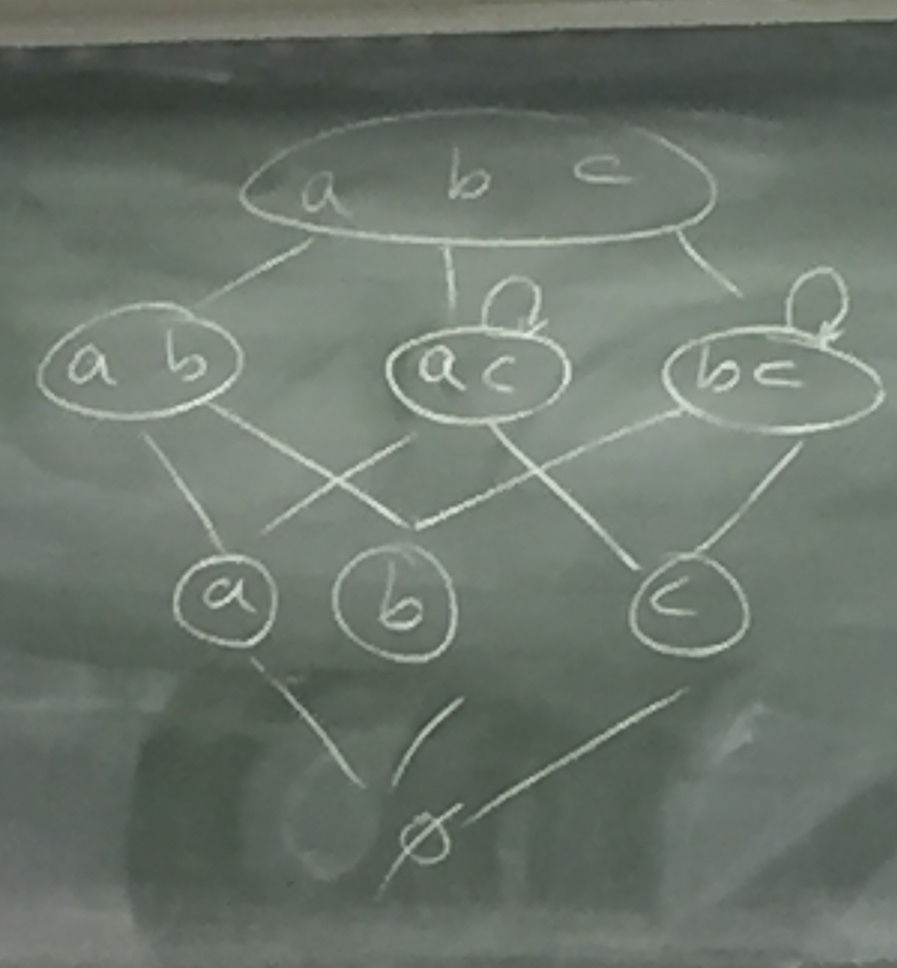
\includegraphics[width=0.7\linewidth]{img/img1}
\caption{}
\label{fig:img1}
\end{figure}
\begin{equation}
\begin{split}
&c \in ac \\
&\tau(c) \subseteq \tau(ac) \\
&\tau(c) = c! \\ % TODO: cancel
&\tau(c) = ac
\end{split}
\end{equation}

\begin{equation}
\begin{split}
&c \in bc \\
&\tau(c) \subseteq \tau(bc) \\
&\tau(c) = c! \\  % TODO: cancel
&\tau(c) = bc
\end{split}
\end{equation}

Dies ist ein Widerspruch


\paragraph{P Datalog-Programm}
$\tau_P$ liefert Fakten von P vereinigt mit Fakten, die in einem Schritt aus der Argumentenmenge von $\tau_P$ mit den Regeln von P abgeleitet werden können.

\subsection*{Ableitung in einem Schritt}

\subsubsection*{Definition: Substitution}
Eine Substitution ist eine endliche Menge der Form
\begin{equation}
\{ X_1 / t_1, \cdots, X_n / t_n \}, X_1,...,X_n \text{ unterschiedliche Variablen, } t_1,....,t_n Terme, X_i \neq t_i
\end{equation}

Falls alle $t_i$ Konstanten sind, ist dies eine \textbf{Grundsubstitution}.

Sei $\theta$ eine Substitution, t ein Term (Variable oder Konstante), so gilt \\

\begin{equation}
t\theta =_{def} \begin{cases} t_i, & \mbox{falls } t/t_i \in \theta \\ t, & \mbox{sonst} \end{cases}
\end{equation}
Sei L ein Literal, $L\theta$ bezeichnet dasjenige Literal, das aus L entsteht, indem alle Variablen $X_i$ mit $L_i$ für die $X_i / t_i \in \theta$ gilt, simultan durch $t_i$ ersetzt werden. Analog $d\theta$ für eine Datalog-Klausel d.

\paragraph{Beispiel}

\begin{equation}
L = p(X, Y, a), \theta = \{X / a, Y / X \} \\
L\theta = p(a, X, a)
\end{equation}

Sei D eine Menge von Datalog Klauseln. In einem Schritt aus D ableitbare Menge von Fakten:

\begin{equation}
fakt_1(D) = \{ f \in HB_D | (\exists Regel L_0 :- L_1,...,L_n)(\exists Sicht \theta)(\{ L_1 \theta, \cdots, L_n\theta \} \subseteq D \wedge f = L_0\theta) \}
\end{equation}

(Annahme: built-in Prädikate geeignet berücksichtigt $\Rightarrow$ Algorithmus FAKT\_1)

Definiere $\tau_P | 2^{HB} \Rightarrow 2^{HB}$. $\tau_P(I) =_{def} P_F \cup fakt_1(P_R \cup I)$.$ P_f = $ Menge der Fakten von P. $P_P$ Menge von Regeln von P.

\subsection*{Satz 1.3} Für jedes Datalog-Programm P ist $\tau_P$ eine monotone Transformation auf $(2^{HB}, \subseteq)$.

\subsubsection*{Beweis}
Seien $I_1, I_2 \in HB_P$ mit $I_1 \subseteq I_2$. z.Z.: $\tau_P(I_1) \subseteq \tau_P(I_2)$. \\
Sei $f \in \tau_P(I_1)$. Falls $f \in P_F$, dann gilt auf $f \in \tau_p(I_2)$. $f \in fakt_1(P_R \cup _1)$ da $I_1 \subseteq I_2$, gilt $P_R \cup I_1 \subseteq P_R \cup I_2$ und somit $f \in fakt_1(P_R \cup I_2)$ wg. Monotonie von Fakt\_1 auf ($2^{HB}, \subseteq$).


\paragraph{Beispiel}

\begin{equation}
\begin{split}
P = &p(1) \\
= &p(2). \\
= &r(1). \\
&\\
q(X) :- &s(X), r(X). \\
s(X) :- &p(X).
\end{split}
\end{equation}

$\leadsto^{T_p(\emptyset)}$

\begin{equation}
\begin{split}
&p_1\\
&p_2 \\
&r_1
\end{split}
\end{equation}

$\leadsto^{T_p(\cdots)}$

\begin{equation}
\begin{split}
&p_1\\
&p_2 \\
&r_1\\
&s(1) (\text{fakt\_1}) \\
&s(2) (\text{fakt\_1})
\end{split}
\end{equation}

$\leadsto^{T_p(\cdots)}$

\begin{equation}
\begin{split}
&p_1\\
&p_2 \\
&r_1\\
&s(1) \\
&s(2) \\
&q(1) (\text{fakt\_1})
\end{split}
\end{equation}

\subsection*{Satz 1.4} Für jedes Datalog-Programm P gilt $cons(P) = lf_p(\tau_p)$ (lf = least fixpunkt).

\subsubsection*{Beweis}:
\paragraph{1)} cons(P) ist ein Fixpunkt von $\tau_P$. \\
$\tau_p(cons(P)) = P_F \cup fakt\_1(P_R \cup cons(P))$. cons(P) ist kleinstes Herbrand-Modell von P, d.h. alle Regeln sind gültig unter $cons(P) \Rightarrow fakt\_1(P_R \cup cons(P) = cons(P) \backslash P_F)$. (und kein Fakt kann aus cons(P) entfernt werden, ohne dass die Modelliereigenschaft verloren geht.) $\Rightarrow \tau_P(cons(P)) = P_F \cup cons(P) \backslash P_F = cons(P)$

\paragraph{2)} $cons(P)$ ist minimaler Fixpunkt von $\tau_P$.\\
Annahme: $(\exists I \not\subseteq cons(P))(\tau_P(I) = I)$.\\
cons(P) ist minimales Herbrand-Modell $\Rightarrow$ I ist kein Herbrand-Modell. Da $P_F \subseteq I$ wg. Annahme $\tau_P(I) = I$ folgt midestens eine Regel ist nicht erfüllt, d.h. $(\exists h_0, \cdot,h_n \in P_R)(\exists Substitution \theta)(\{ h_1\theta, \cdots, L_n(\theta)\} \subseteq I \wedge L_1 \theta \cancel{\in} I)$. Aber $L_0 \in fakt_1(P_R \cup I)$ nach Definitio von fakt\_1.
Da auch $L_0 \theta \in P_F$ wegen $P_F \subseteq I, folgt \tau_P(I) \neq I$. Noch Fixpunkttheorem (Kuaster / Tarski) ist minimaler Fixpuknt von $\tau_P$ kleinster Fixpunkt von $\tau_P$. 

\subsection*{Vorgehensweise bei Fixpunktberechnung} bottom-up

\subsubsection*{Bezeichnung: Forward-chaining}Da ``$\Leftarrow$'' die natürliche Richtung für die Anwendung von Regeln ist.
Da Regeln sicher sind ist $L_i \theta$ stets ein Fakt $\theta_i$.
Betrachte Eignung der Methode zur Anfrageauswertung, z.B. ?- vs(c4, y). ``Alle Kurse, die Voraussetzung von Kurs c4 sind''

\paragraph{Ineffizient} Berechnung des $lf_p$ und anschließende Siche zu vs(c4, y) passende Fakten $\Rightarrow$ Vermeide möglichst Berechnung nicht relevanter Fakten (später).

Starte mit Zielklausel, Suche ein Regel die zu einem Atomder Klausel passt. Ersetze das Atom durch angepassten Rumpf der gewählten Regel, neue Anfrage, iterieren.

\subsubsection*{Bezeichnung: Backward-chaining}
\paragraph{Beispiel}
\begin{equation}
\begin{split}
P = &p(1) \\
= &p(2). \\
= &r(1). \\
&\\
q(X) :- &s(X), r(X). \\
s(X) :- &p(X).
\end{split}
\end{equation}

% TODO: img 3 hier


\subsection*{Prozedurale Semantik}
Beweistheoretische Sicht, übertragen auf Datalog Programm P aufgefasst als Theorie 1. Stufe \\
Semantik: $\{f \in HB_P | P \vdash f \}$ \\
Wie können Ableitungen (Beweise) von Fakten systematisch durchgeführt werden?

Regeln: 
\begin{equation}
\begin{split}
(1) vs(X, Y) &:- Kp(X, Y). \\
(2) vs(X, Y) &:- vs(X, Z), kp(Z, Y). \\
P &= \{ Kp (c4, a3), \cdots, kp(c2, a0), (1), (2) \} 
\end{split}
\end{equation}

Zeige $P \vdash vs(c4, a0)$. 
\begin{equation}
\begin{split}
(1) = (\forall X)(\forall Y)&(kp(X, Y) \Rightarrow vs(X, Y)) \\
(2) = (\forall x)(\forall Y)(\forall Z)&(vs(X, Z) \wedge kp(Z , Y) \Rightarrow vs(X, Y))
\end{split}
\end{equation}

\paragraph{Beweis}
\begin{figure}
\centering
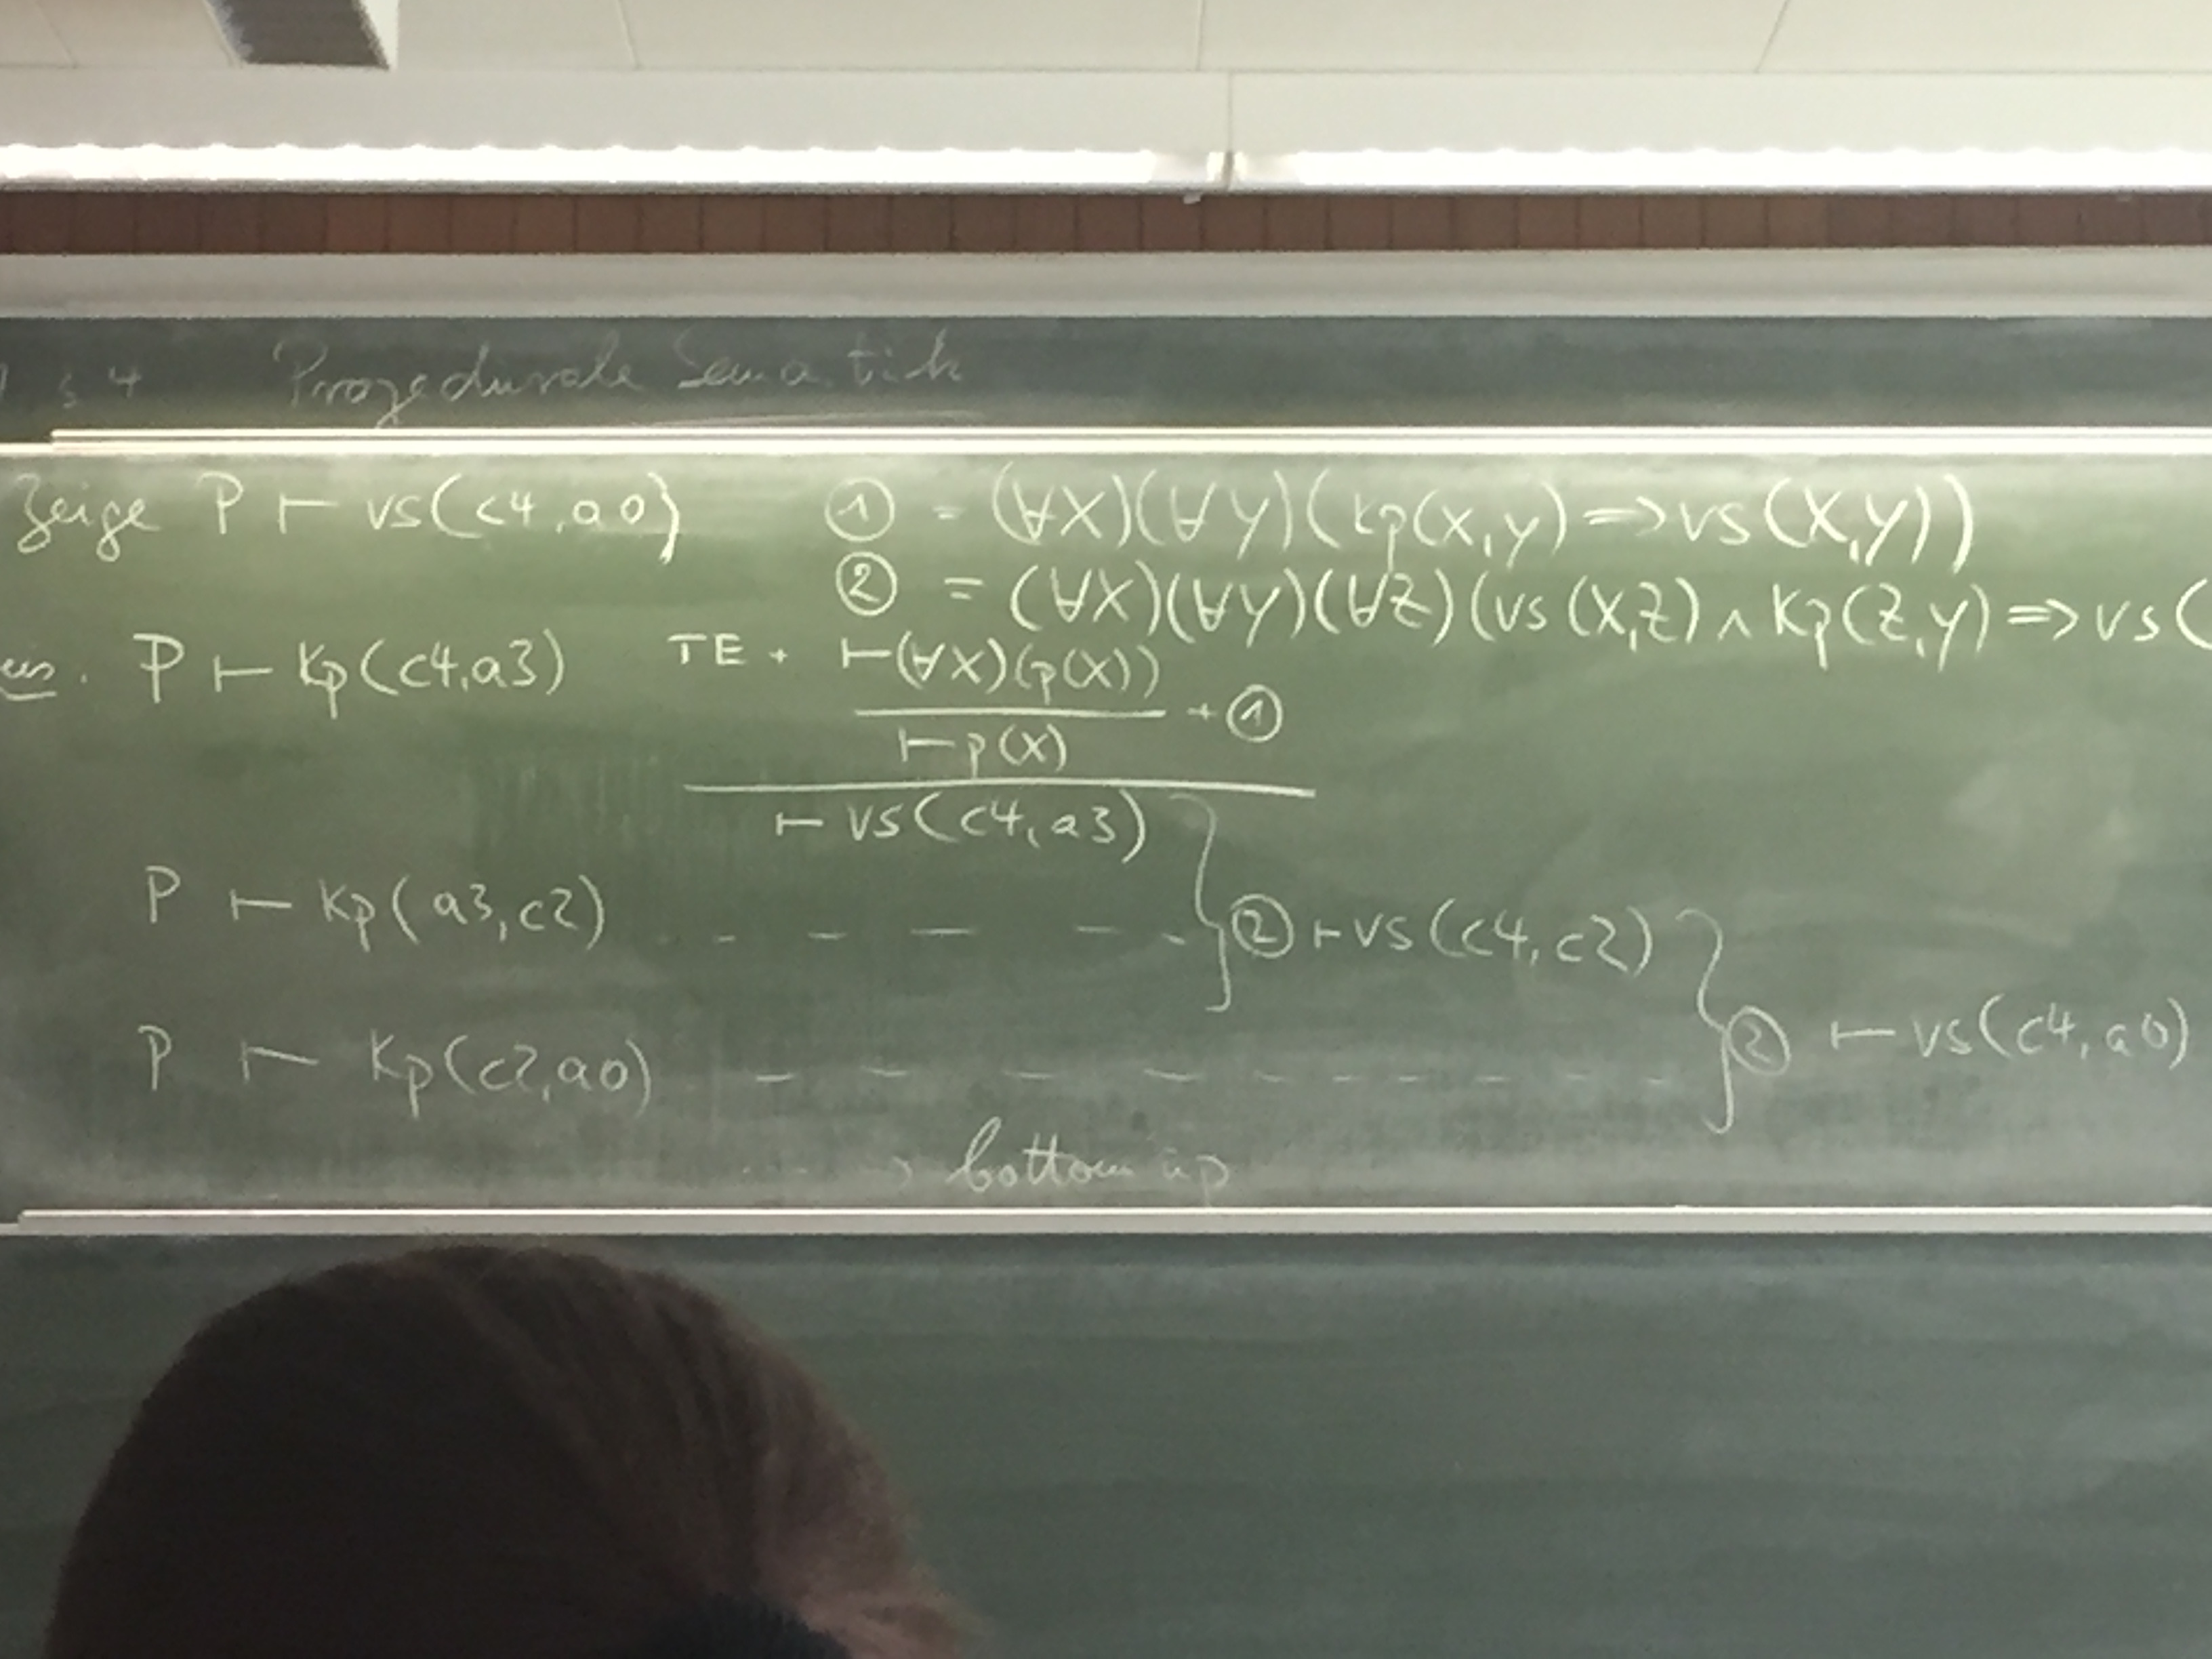
\includegraphics[width=0.7\linewidth]{img/img4}
\caption{}
\label{fig:img4}
\end{figure}
\begin{figure}
\centering
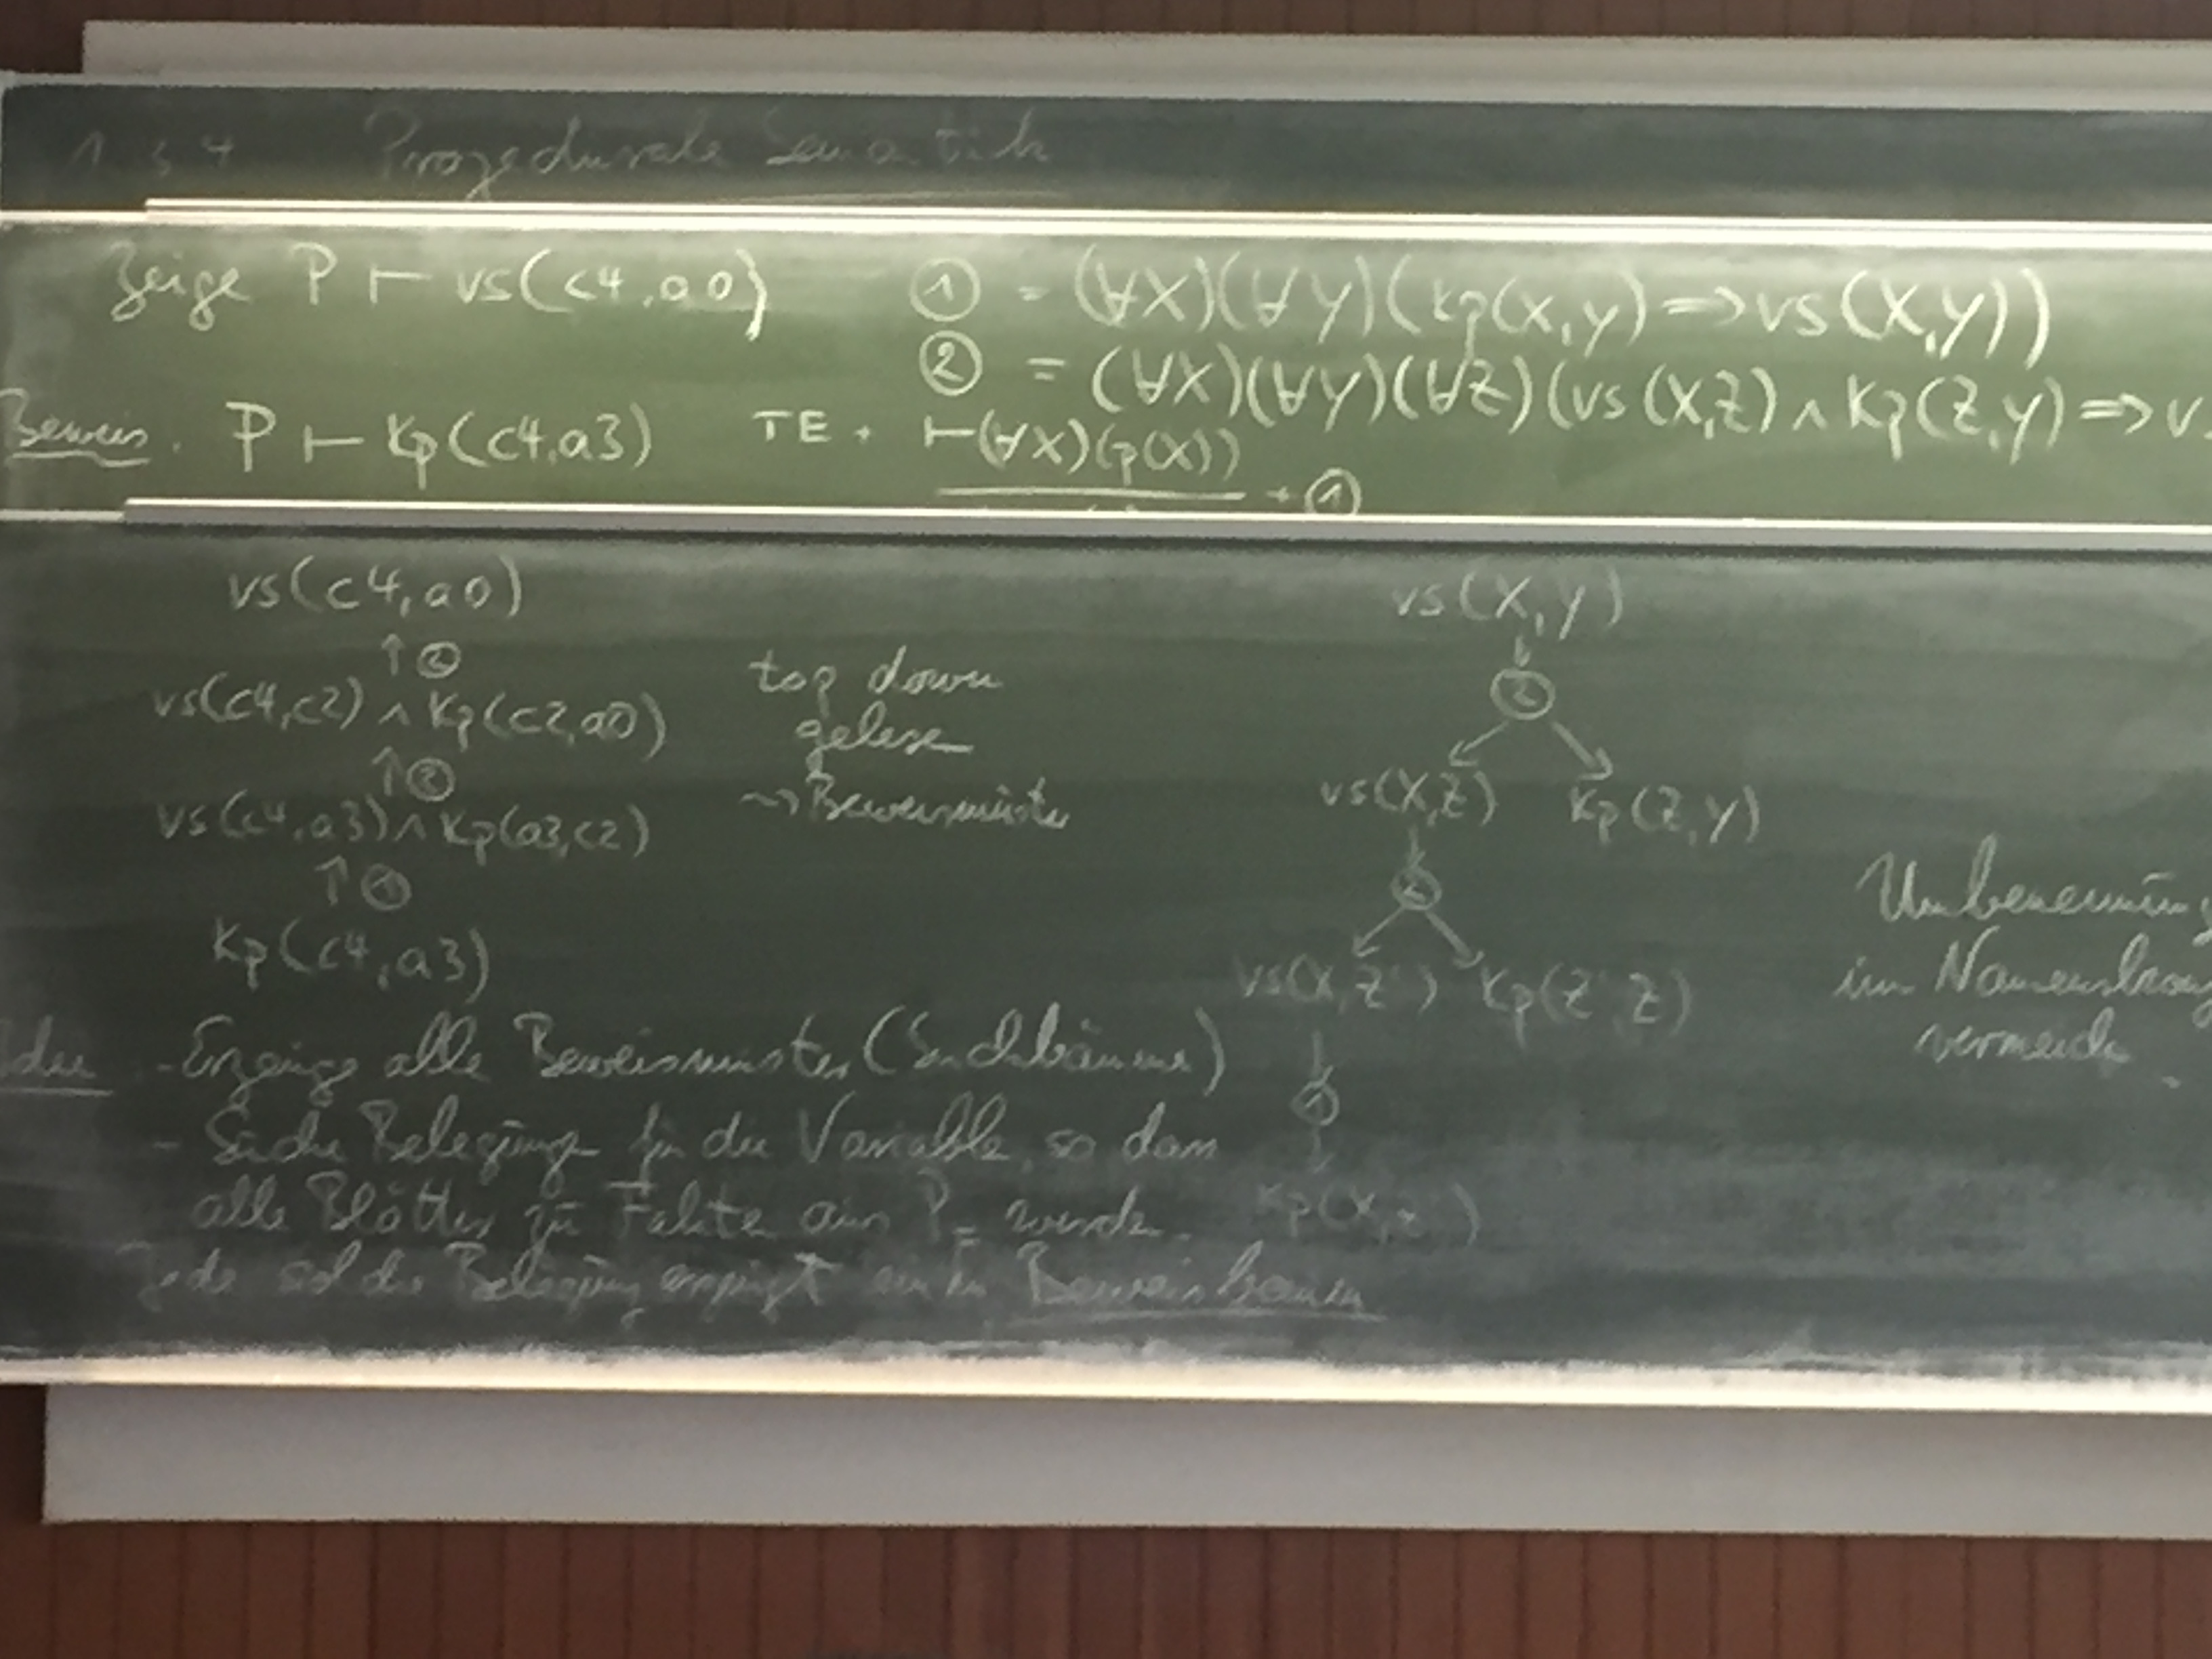
\includegraphics[width=0.7\linewidth]{img/img5}
\caption{}
\label{fig:img5}
\end{figure}

\paragraph{Idee} 

\begin{itemize}
\item Erzeuge alle Beweismuster (Suchbäume)
\item Suche Belegungen für die Variable, so dass alle Blätter zu Fakten aus P werden
\item jede solche Belegung erzeugt einen Beweisbaum.
\end{itemize}

\paragraph{Zunächst} Suche nach ``passenden'' Köpfen von Regeln erfordert Definition.

\subsubsection*{Definition: Unifizierbar}

Seien $L_1$ und $L_2$ heißen \textbf{unifizierbar}, wenn $(\exists \text{ Substitution } \Theta)(L_1\Theta = L_2\Theta)$. $\Theta$ heißt dann \textbf{Unifikator}.

\paragraph{Beispiel}

$L_1 = vs(X, Z)$ \\
$L_2 = cs(X, Y)$ \\
$\Theta = \{ Z / Y \}$ und $\Theta = \{ Y / Z \}$ sind Unifikatoren von dem Paar $L_1, L_2$, aber auch $\Theta = \{ X/a, Y/a, Z/a \}$. Die ersten beiden sind spezifischer als das letzte

$L_1 = q(X, Y ,c) L_2 = q(W, b, Z)$
Unifikation z.B.:
\begin{equation}
\begin{split}
\Theta_1 &= \{ X/W Y/b Z/c \} \\
\Theta_2 &= \{ X/T, W/T, y/b, Z/c \} \\
\Theta_3 &= \{ X/a, W/a, Y/b, Z/c\}
\end{split}
\end{equation}

Nicht unifizierbar:
$L_1 = q(X, c, U) L_2 = q(W, G, Z)$ oder $L_1 = q(X, a, X) L_2 = q(b, Y, Y)$

\subsubsection*{Definition: Komposition}

Sei $\Theta = \{ X_1 / t_1, \cdots, X_n / t_n \}, \varsigma = \{ Y_1 / n_1, \cdots, Y_m / t_m \}$ Substitutionen. \\
Die Komposition $\Theta\varsigma$ von $\Theta$ und $\varsigma$ erhält man aus 
\begin{equation}
X_1 / t_1\varsigma, \cdots, X_m / t_m\varsigma, Y_1 / n_q, \cdots, Y_m / n_m
\end{equation}
Durch Streichen von Elementedn der Form Z/Z sowie $Y_i / n_i$ mit $Y_i = X_j$ für ein j$j \in \{1, ..., n\}$

\paragraph{Beispiel} $\theta= \{ X/a,  Y/W \} \varsigma=\{X/ bm Y/ V, W/Z \}$ \\
$\Theta\varsigma = \{ X/a, YZ, W/Z \}$

\subsubsection*{Definition: allgemeinere Substitution}
Seien $\Theta, \varsigma$ Substitutionen, $\Theta$ heißt allgemeiner als $\varsigma \diamondsuit (\exists \text{Substitution} \delta)(\Theta \delta = \varsigma)$.
Seine $L_1, L_2$ Literale. Ein allgemeinster Unifikator (mgu) von $L_1 in L_2$ ist ein Unifikator von $L_1 und L_2$, der allgemeiner als alle anderen Unifikatoren ist.

\paragraph{Beispiel} $\Theta_2$  ist allgemeiner als $\Theta_3$; betrachte $\delta = \{T / a\}$, es gilt $\Theta_2\delta = \Theta_3$. $\Theta_1$ ist allgemeiner als $\Theta_2, \delta = \{ W / T \}$. mgu ist i.A. nicht eindeutig bestimmt. $L_1 = p(X,X) L_2 = p(V,W)$
mgu: \\
\begin{equation}
\begin{split}
&\{ X/W, V/W \} \\
&\{ X / V, W/V\} \\
&\{ V/X, W/X \}
\end{split}
\end{equation}

\paragraph{Beispiel}
$L_1 = q(X,Y,c)\footnote{t1, t2, t3} L_2 = q(W, b, Z) \footnote{k1 k2 k3}$ \\
\begin{figure}
\centering
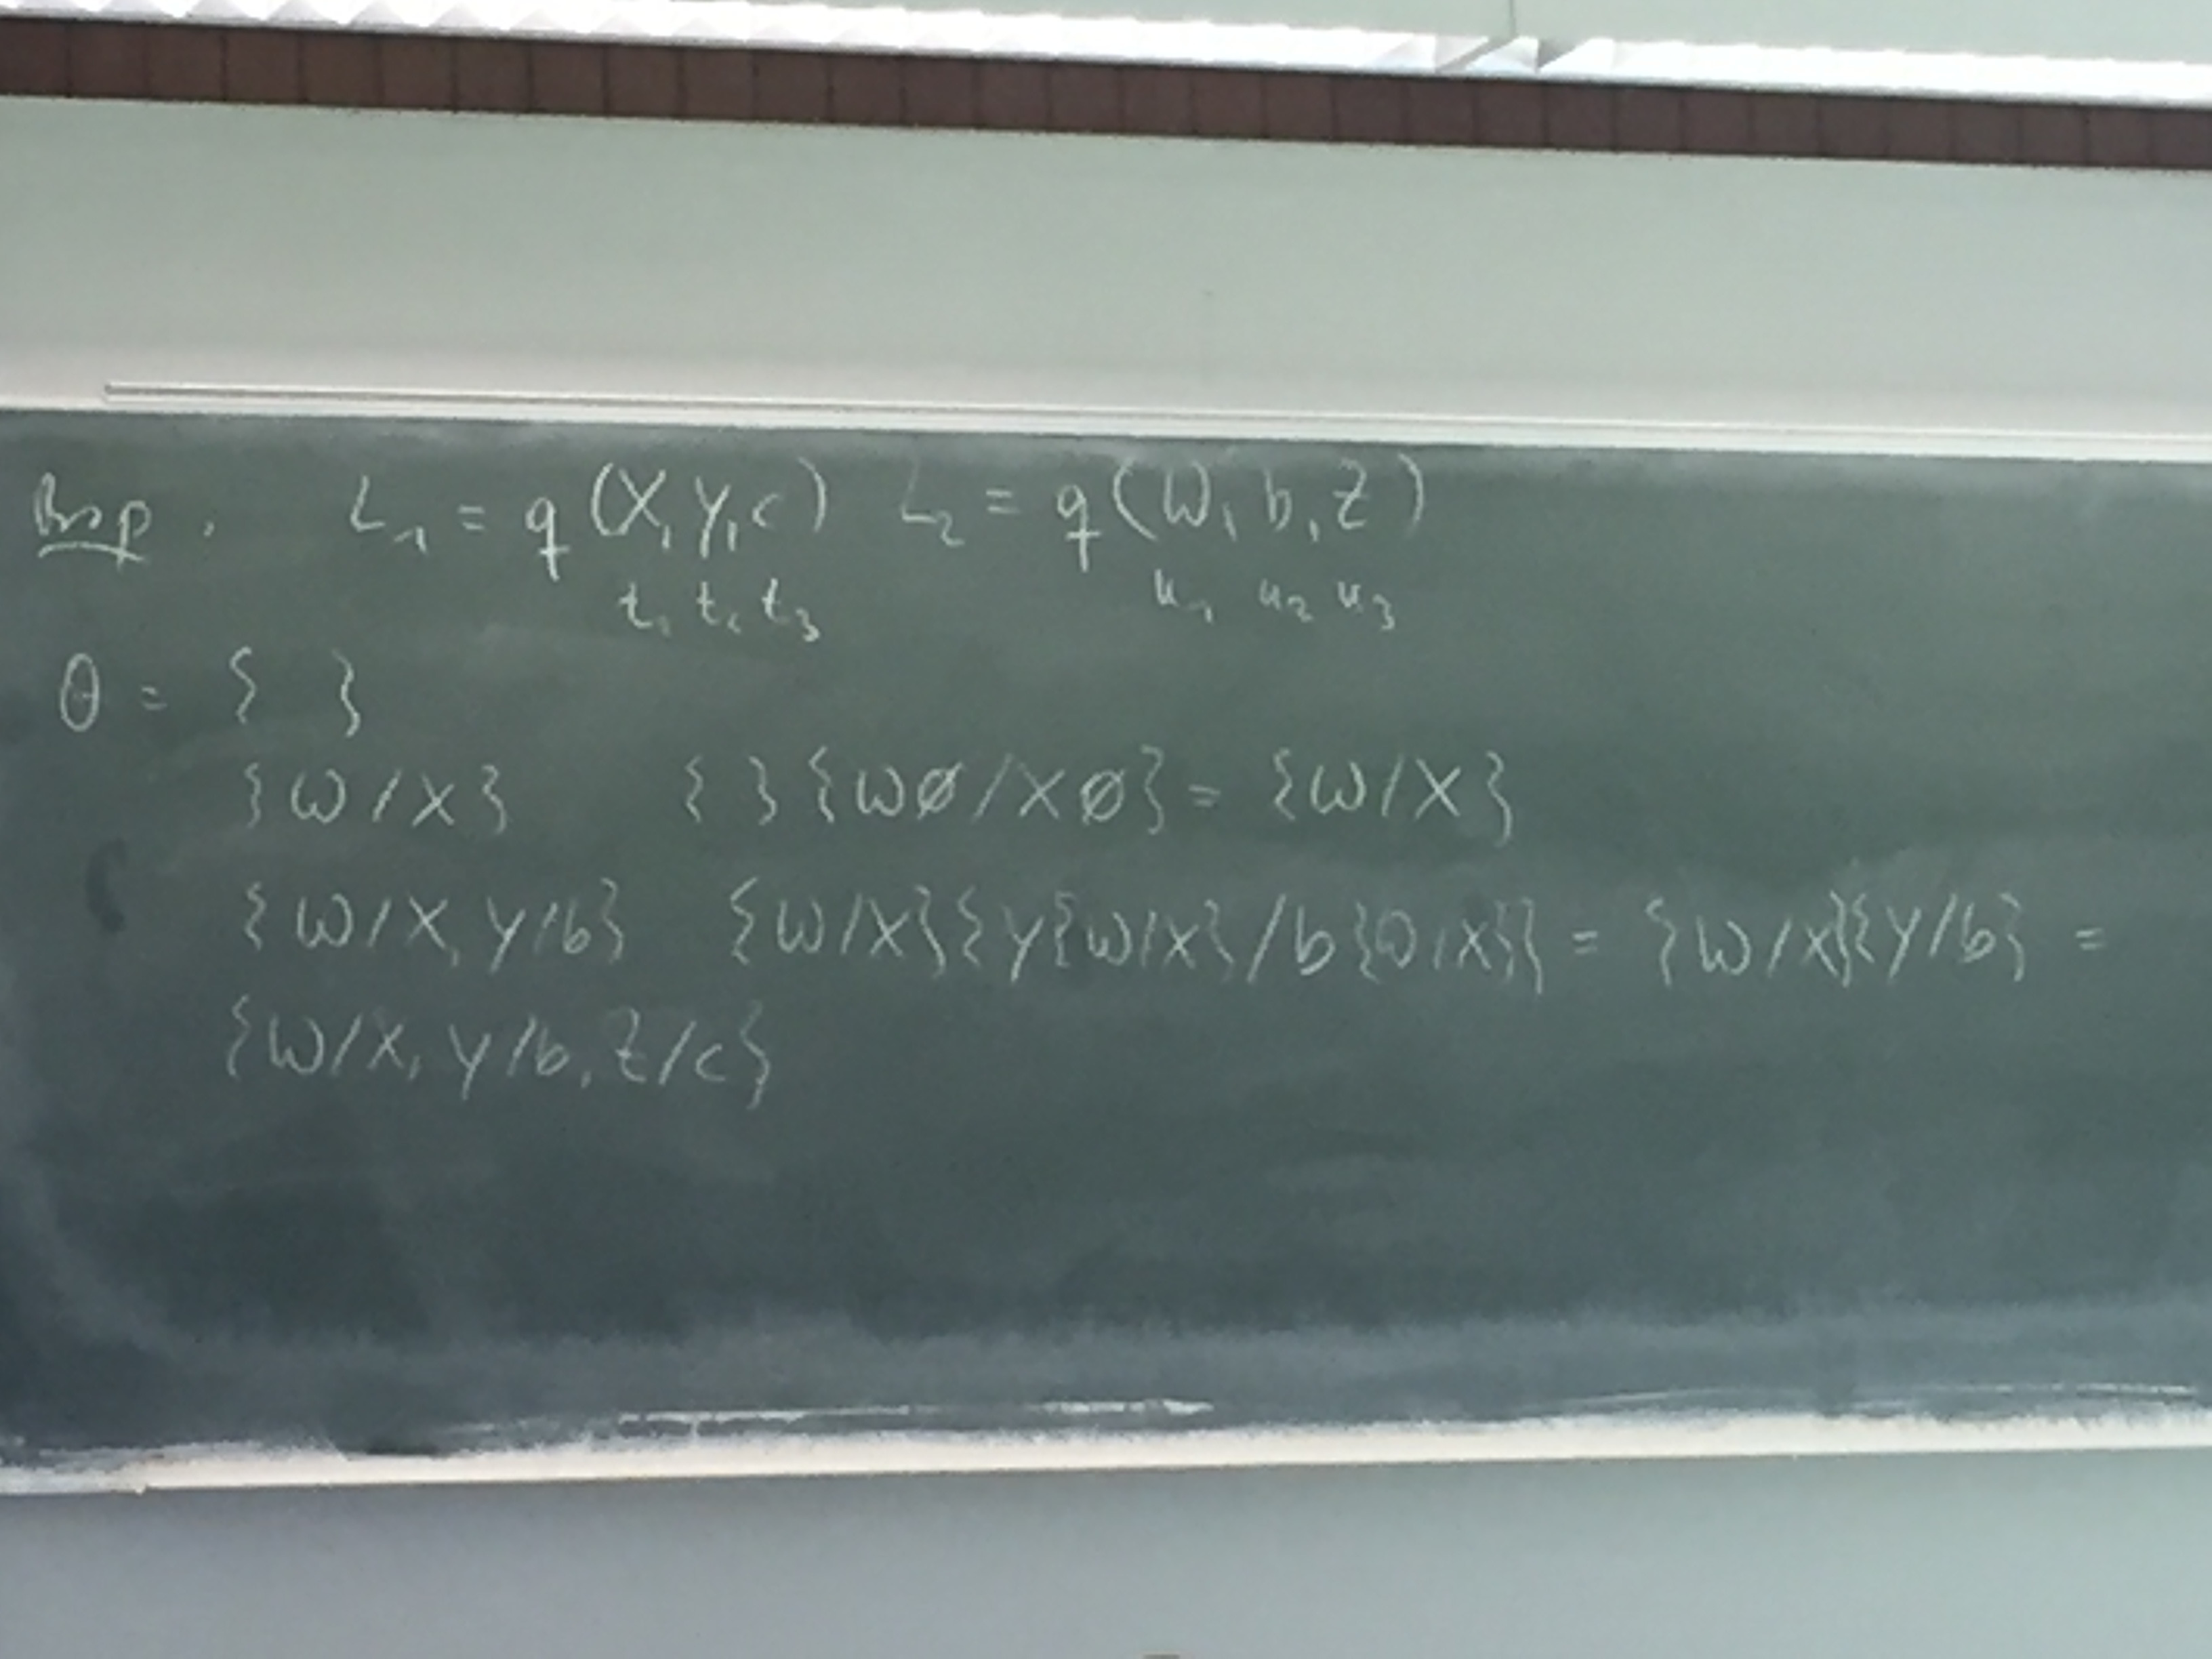
\includegraphics[width=0.7\linewidth]{img/img6}
\caption{}
\label{fig:img6}
\end{figure}


\subsection*{Suchbaum} (Beweismuster zu einem Programm P)
\begin{itemize}
\item Wurzel ist mit einem ``Ziel'' $g = p(t_1, \cdots, t_n), p \in iPr\ddots{a}d$, bekannt.
\item Knoten entlang eines Pfades von der Wurzel aus sind abwechselnd mit Atome und Regeln benannt. (Ziel-, Regelknoten)
\item Alle Blattknoten sind mit Atomen benannt
\item Sei k ein mit einem Atom $a(s_1,...,s_l)$ benannten Knoten (keine Blattknoten), dann ist der unmittelbare Nachfolger von k mit einer Regel von P benannt, deren Kopf mit $q(sq, ..., s_l)$ unifizierbar ist
\item sei k' ein mit einer Regel $r = L_0 :- L_1,...,L_m$ benannte Knoten der unmittelbare Vorgänger von k' sei mit $q(s_1,...,s_l)$ benannt. Dann hat k' m unmittelbare Nachfolger, die mit $I_1 mgu(q(s_1, ..., s_l), I_{0}^{~}), ..., I_m mgu(q(s_1,...,s_l), I_0)$ benannt sind. Dabei sind $I_0, .., I_m$ Atome, die aus $L_1,...,L_m$ durch eventuelle Umbenennung von Variablen hevorgehen (die Variablen seien stets so umbenannt, dass sie im Baum eindeutig sind).
\end{itemize}

\paragraph{Beispiel}
\begin{figure}
\centering
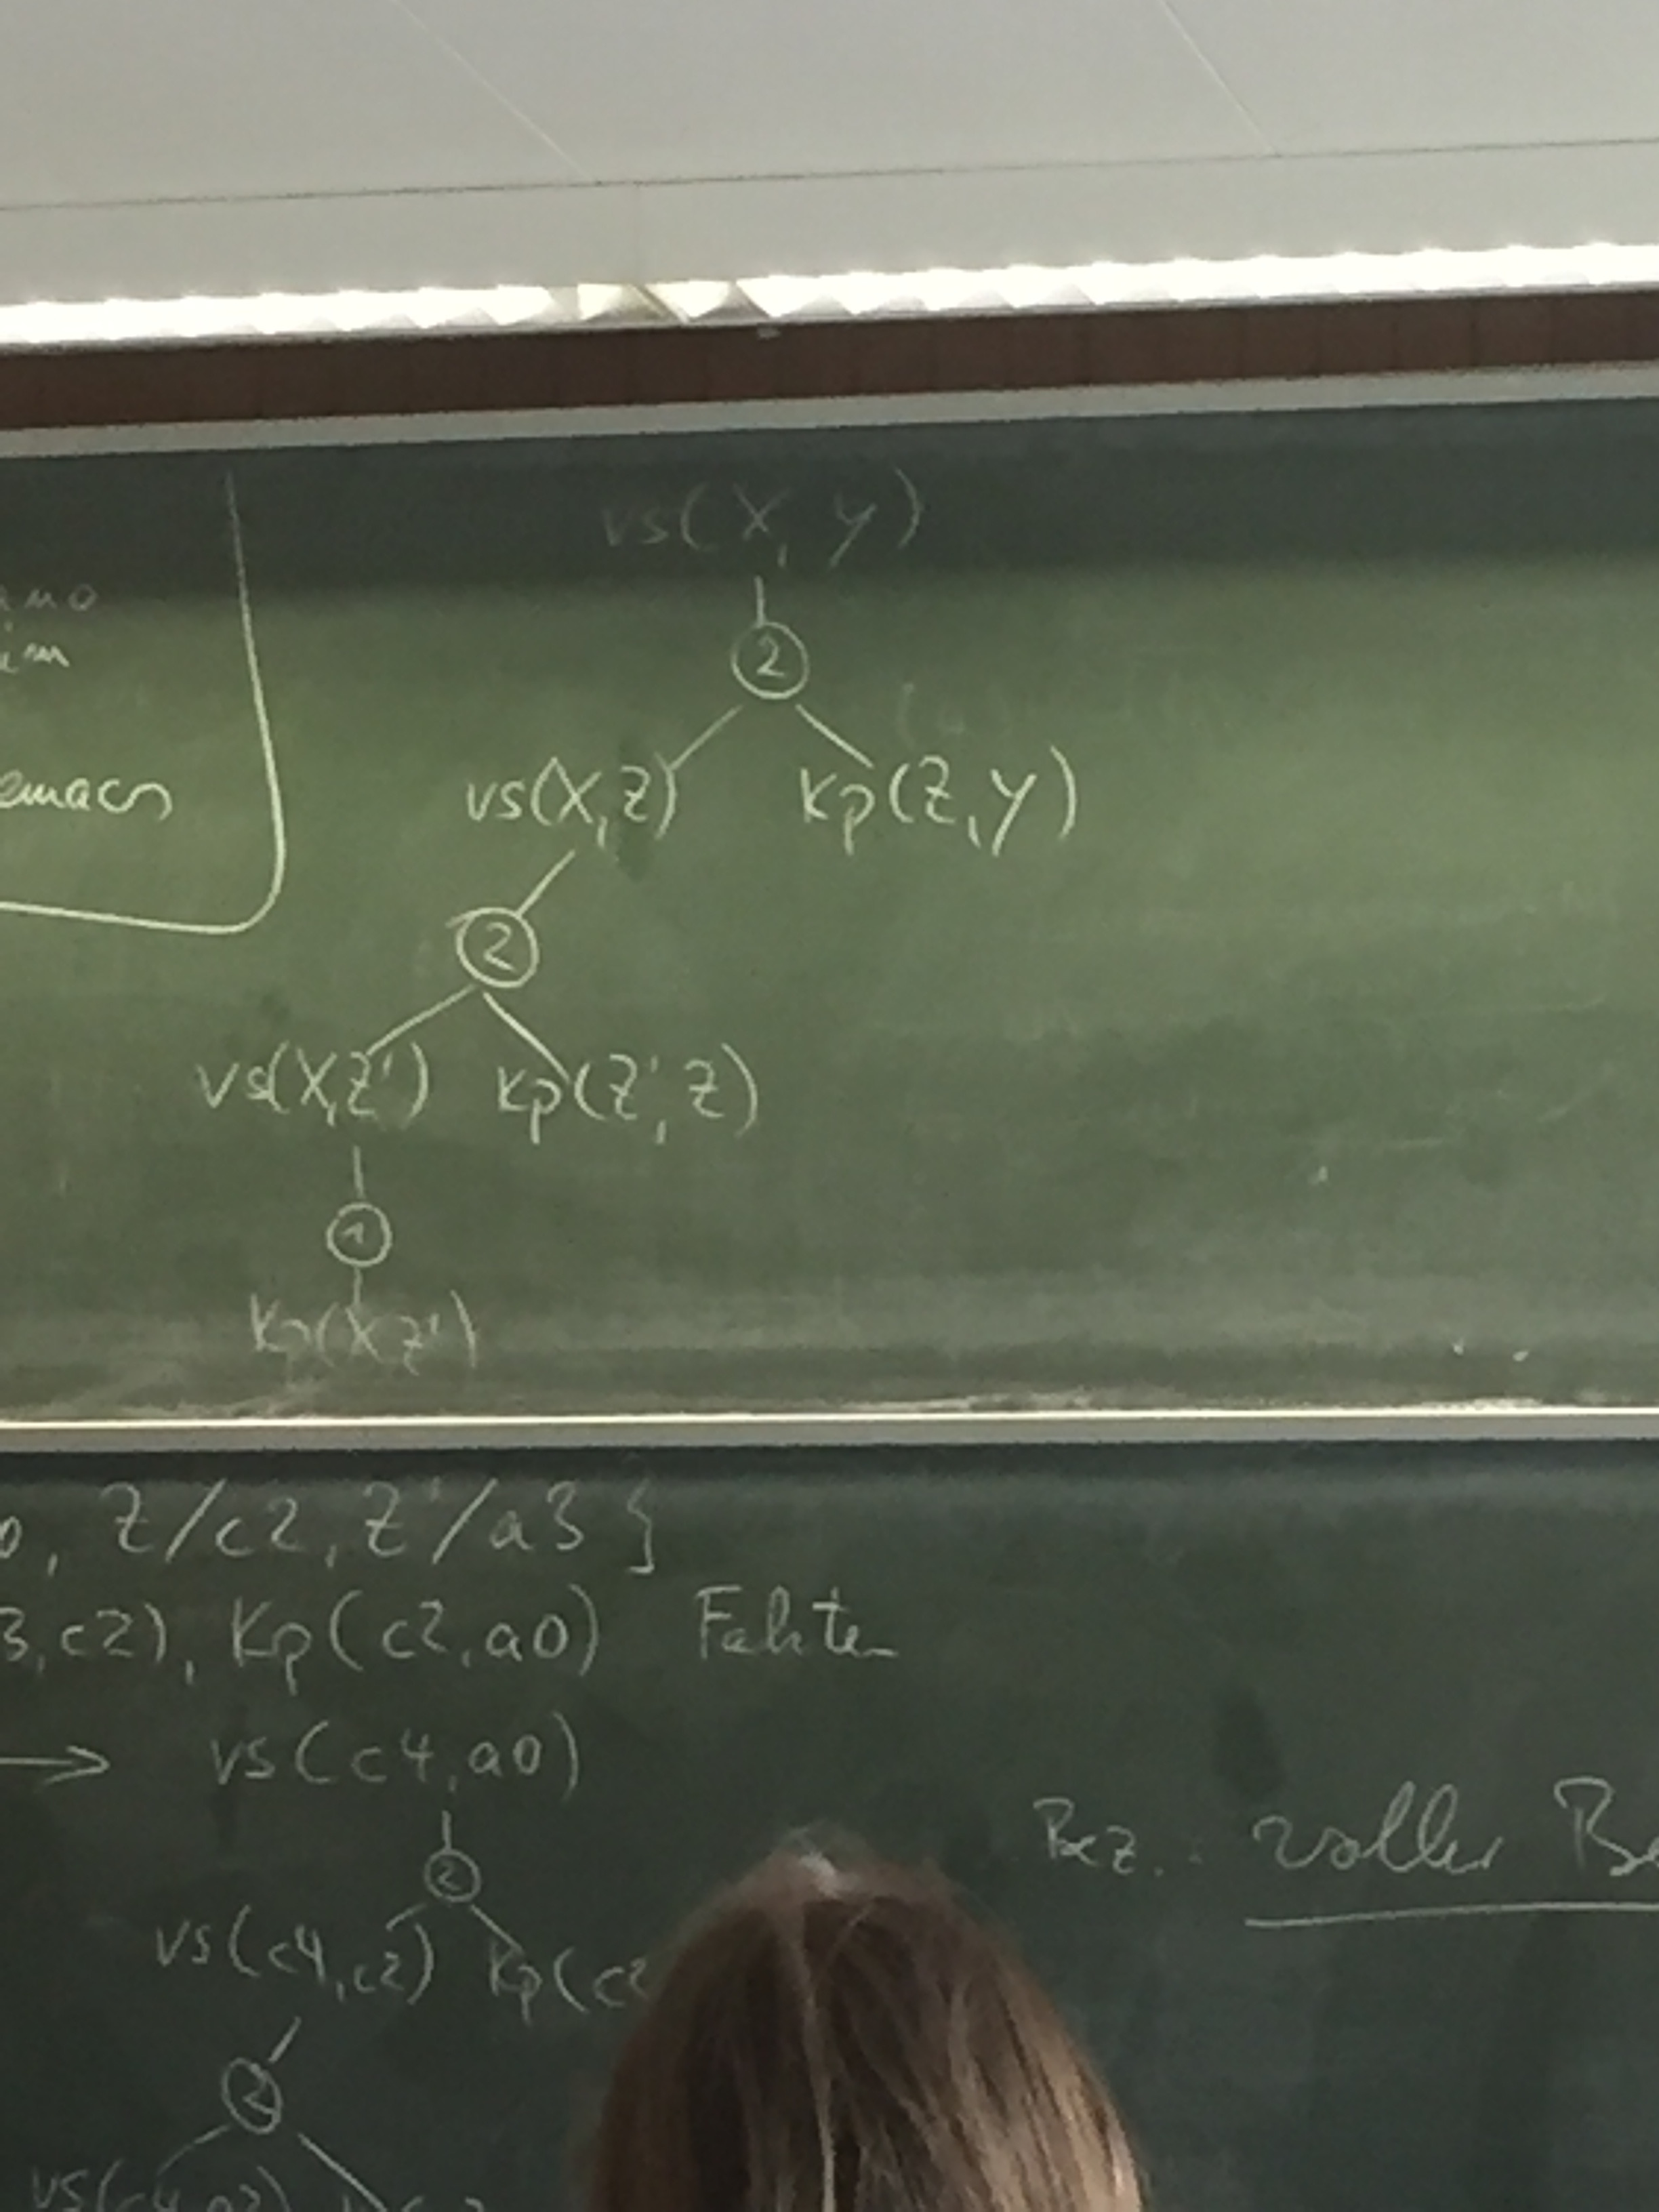
\includegraphics[width=0.7\linewidth]{img/img7}
\caption{}
\label{fig:img7}
\end{figure}

\subsubsection*{Suchbaum $\rightarrow$ Beweisbaum}
Gegeben Sei der Suchbaum S und eine Grundsubstitution $\Theta$ mit folgenden Eigenschaften:
\begin{itemize}
\item $\Theta$ ordnet jeder Variable in S ein Konstantensymbol aus der Menge der in P vorkommenden Konstantensymbole zu.
\item Für jedes Blatt von $S$ gilt, dass $\Theta$, angewand auf die Benennung des Blattes, einen Fakt aus $P_F$ liefert (build-in-Prädikate seien entsprechend berücksichtigt)
\end{itemize}

\paragraph{Beweisbaum} B entsteht aus S durch Anwendung von $\Theta$ auf alle Benennungen von Zielknoten. B repräsentiert einen Beweis für $g\Theta$, g benennung der Wurzel von S.

\paragraph{Beispiel:}
\begin{align*}
\Theta &= \{ X / c4, Y / a0, Z c2, Z'/ a3 \} \\
&kp(c4,a3), kp(a3, c2), kp(c2, a0)  \text{ Fakten}\\
\end{align*}

\begin{figure}
\centering
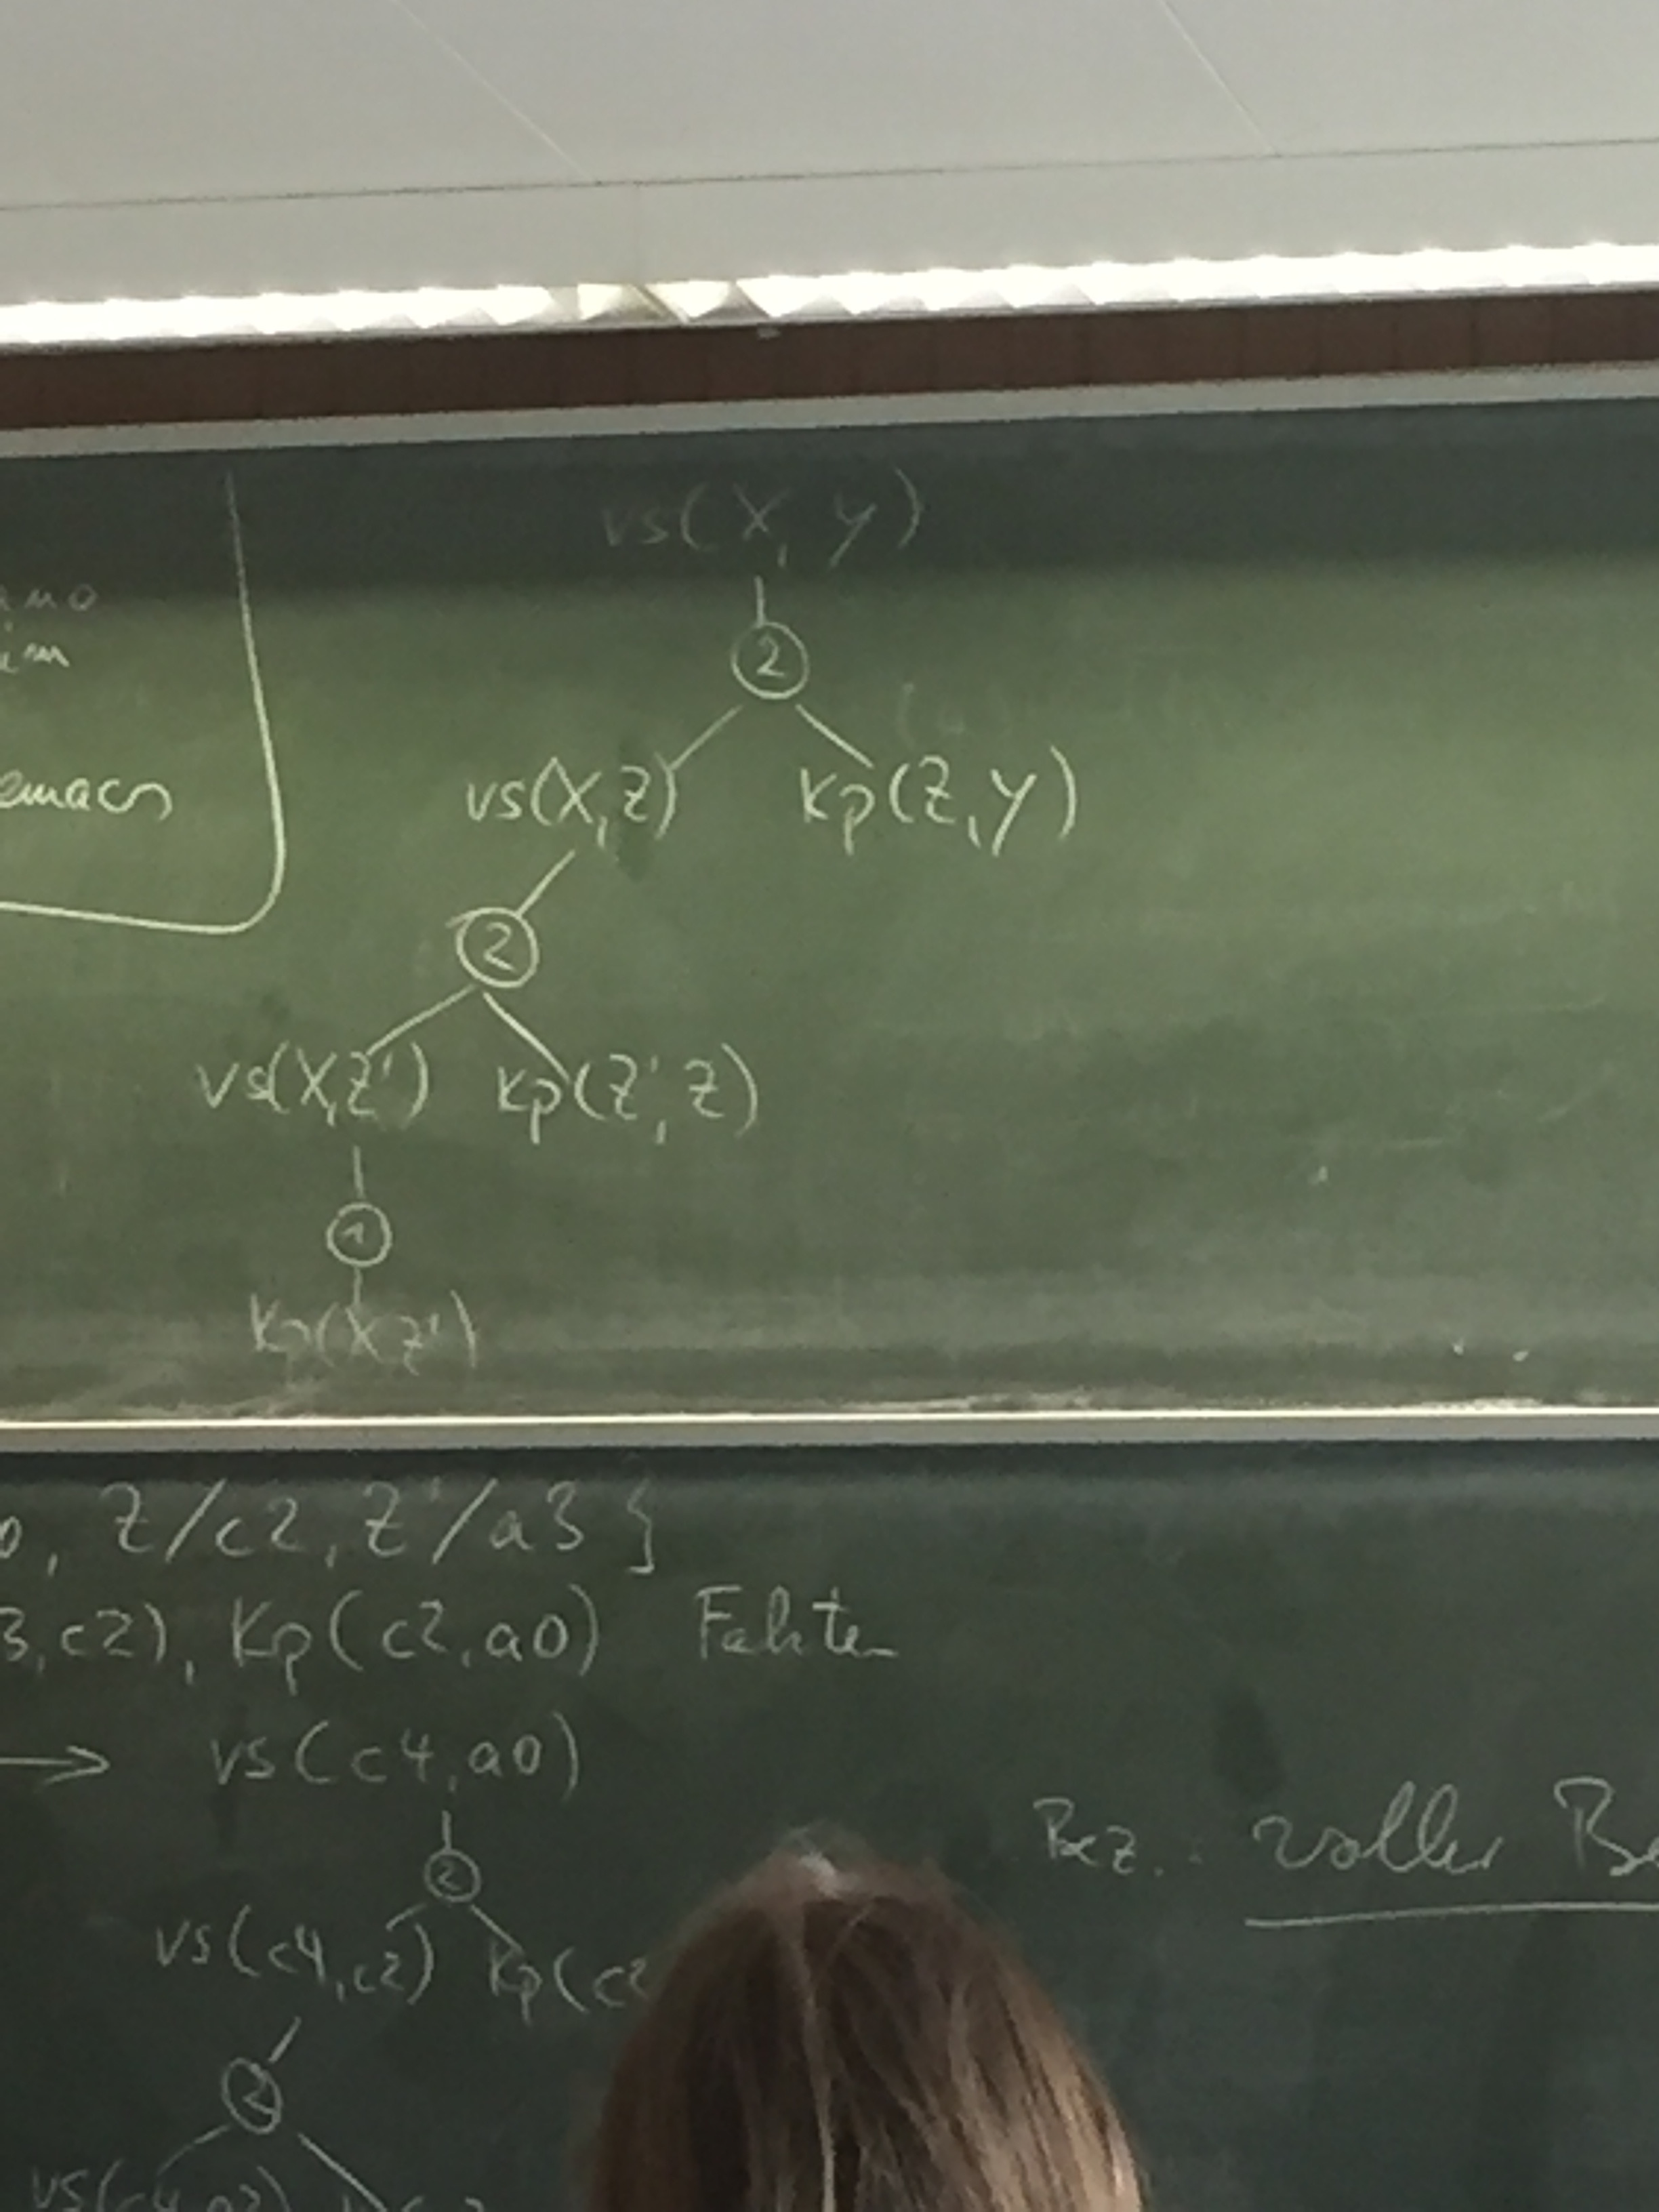
\includegraphics[width=0.7\linewidth]{img/img7}
\caption{}
\label{fig:img7}
\end{figure}

\paragraph{Bezeichnung}: Voller Beweisbaum

\subsubsection*{Systematische Erzeugung der Suchbäume}
Sukzessive alle Bäume der Tiefe 1,2, ... Erzeugen (breadth first)

\paragraph{Definition: Tiefe eines Baums} maximale Anzahl von Zielknoten auf einem Pfad von einem Blattknoten zur Wurzel. Entsprechend Knoten der Tiefe i, Ebene i eines Baumes. Zusätzlich: Spezielle Suchbäume (Tiefe 0) für Fakten aus P.

\paragraph{Beispiel}: Ziel $g = vs(c4, y)$ \\

\begin{itemize}
\item \textbf{Tiefe 1}: vs(c4, y), $\Theta$, kein Beweisbaum
\item \textbf{Tiefe 2}: vs(c4, y)  \\
kp(c4,y), $\{ y / a3 \}$
\end{itemize}

% TODO: Insert Image 8

\paragraph{Offensichtlich}
\begin{itemize}
\item Zu jedem endlichen Beweise, der mit Grundatomen ``Startet'', kann ein entsprechender Beweisbaum auf den beschriebenen Weg erhalten werden.
\item Zu jedem Fakt  $f \in cons(P)$ gibt es einen endlichen Beweis, der mit Grundatomen startet, siehe Fixpunktberechnung $\rightarrow$ voller Beweisbaum
\end{itemize}

$\Rightarrow$ Methode Suchbaum / Beweisbaum ist vollständig. \\
Da ein Beweisbaum mit $g\Theta$ als Benennung der Wurzel einen Beweis für $g\Theta$ darstellt $\Rightarrow$ Methode Suchbaum / Beweisbaum ist korrekt.


\subsection*{Satz 1.5} Sei P ein Datalog-Programm. Die Suchbaum  / Beweisbaum Methode, angewand auf alle Ziele $q(X_1, \cdots, X_{Stelligkeit(q)})$, q intentionales Prädikatesymbol von P, liefert cons(P) als Ergebnis

\paragraph{Frage:} Abbruchkriterium bei der Erzeugung von Suchbäumen

Es gilt
\begin{itemize}
\item Beweisbäume sind isomorph zu den Suchbäumen, aus denen sie erzeugt wurden
\item Zu jedem Fakt $f \in cons(P)$ gibt es einen vollen Beweisbaum, in dem auf jeder Zielknotenebene ein neuer Fakt (neues Teilziel) auftritt
\paragraph{Beweis}
Sei B ein voller Beweisbaum, der diese Eigenschaft nicht erfüllt.
Dann gibt es ein i, so dass in B auf Ebene i nur Fakten auftreten, die schon auf vorhergehenden Ebenen auftreten. Die Teilbäume von B mit Wurzel auf Ebene i können ``höher gehängt'' werden $\Rightarrow$ Es gibt einen äquivalenten, vollen Beweisbaum mit geringerer Tiefe.

\item Es gibt nur endlich viele verschiedene Grundatome, die aus den Prädikaten und Konstantensymbolen gebildet werden können. Konkret: Seien ap(p) die Anzahl verschiedener Prädikatensymbole die in p vorkommen
\item ak(p) die Anzahl verschiedener Konstantensymbole, die in P vorkommen
\end{itemize}

Dann ist $max. fakt(P) = ap(P) * ak(P)^{max\_st(P)}$ eine obere Schranke für die Anzahl verschiedener Grundatome. \textbf{Damit:}
	
\subsubsection*{Satz 1.6} Die Suchbaum / Beweisbaum Methode bleibt vollständig für ein Programm P, wenn nur Bäume mit max. Tiefe max\_fakt(P) betrachtet werden.
Statt breadth first andere Vorgehensweise denkbar:

\begin{itemize}
	\item Depth first mir Abbruch bei max\_fakt(P) und backtracking
	\item Dynamische Abbruchbedingungen, abhängig von erzeugten Faktenmenge (limit 10)
	\item Erkennen und Ausnutzen identischer (Teil-) Zielknoten ($\leadsto$ gerichteter, azyklischer Graph)
\end{itemize}

Zusammenfassen von Such und Beweisbäumen, Berücksichtigung von Fakten aus $P_F$ $\Rightarrow$ frühzeitiges Erkennen von Suchbäumen zu denen keine Beweisbäume existieren

\begin{figure}
\centering
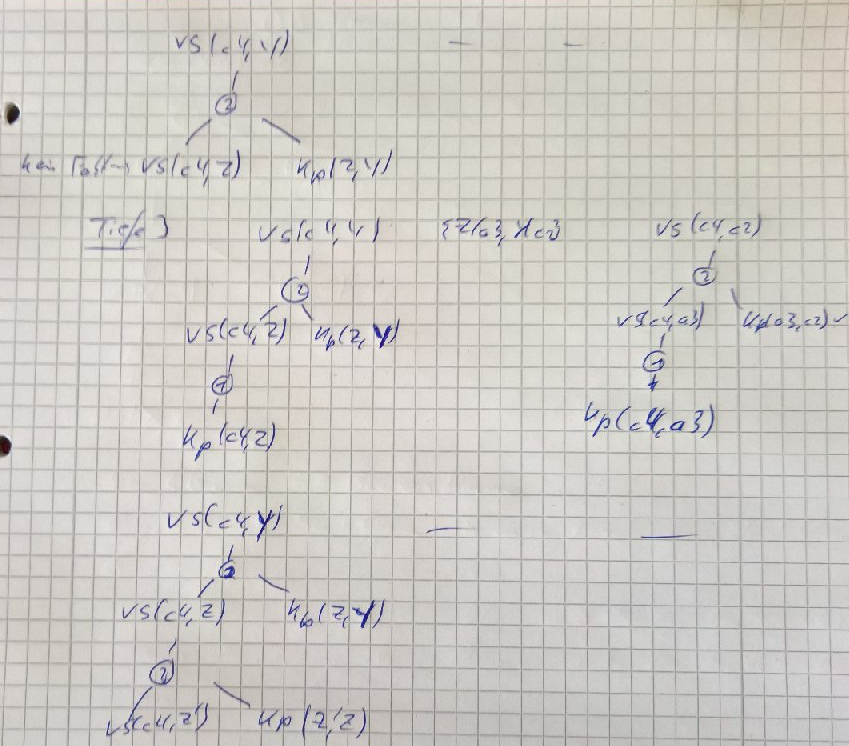
\includegraphics[width=0.7\linewidth]{img/img8}
\caption{}
\label{fig:img8}
\end{figure}

Sei g das Ziel (Wurzelbenenung), dann erzeugt ein Baum der mit der leeren Menge endet, genau ein Ergebnis. 
\begin{align*}
&g \Theta_1, ..., \Theta_n, (\Theta_1, ...., \Theta_n \text{die in dieser Reihenfolge angewandten Unifikatoren (von der Wurzel aus)} \\
&\Theta = \Theta_1, ..., \theta_n \text{ heißt Antwortsubstitution.}
\end{align*}

\subsection*{Resolutionsmethode}

Für allgemeine Klauselformen entwickelte Methode zum automatischen Beweisen.
\paragraph{Literatur} J Allen Robinson: A machine-oriented logic base on the resolution principle. Journal of the ACM 12, S.23-41, 1965 \\

In Logikprogrammierung (Horn-Klauseln): SLD-Resolution (Linear Resolution with Selected Function for Definite Clauses).

\begin{itemize}
\item S (Selection function): Legt fest, wie Literale aus einem Ziel (Klausel mit einem oder mehreren negierten Literalen) auszuwählen sind
\item L (Linear): In jedem Schritt wird genau ein Literal ausgewählt für die Unifikation mit dem Kopf einer Regel einer einem Fakt
\item D (Definit): Beschränkung auf Programme mit definiten Klauseln
\end{itemize}

\paragraph{Bemerkung} Methode steht für ganze Klasse von Algortihmen. Methode auch bekannt unter LUSH (Linear resolution with Unrestricted Selection function for Horn clauses) \\
\paragraph{Übergang Such / Beweisbaum $\leadsto$ Resolution}
Nachweis der Unerfüllbarkeit einer Klausel

\begin{figure}
\centering
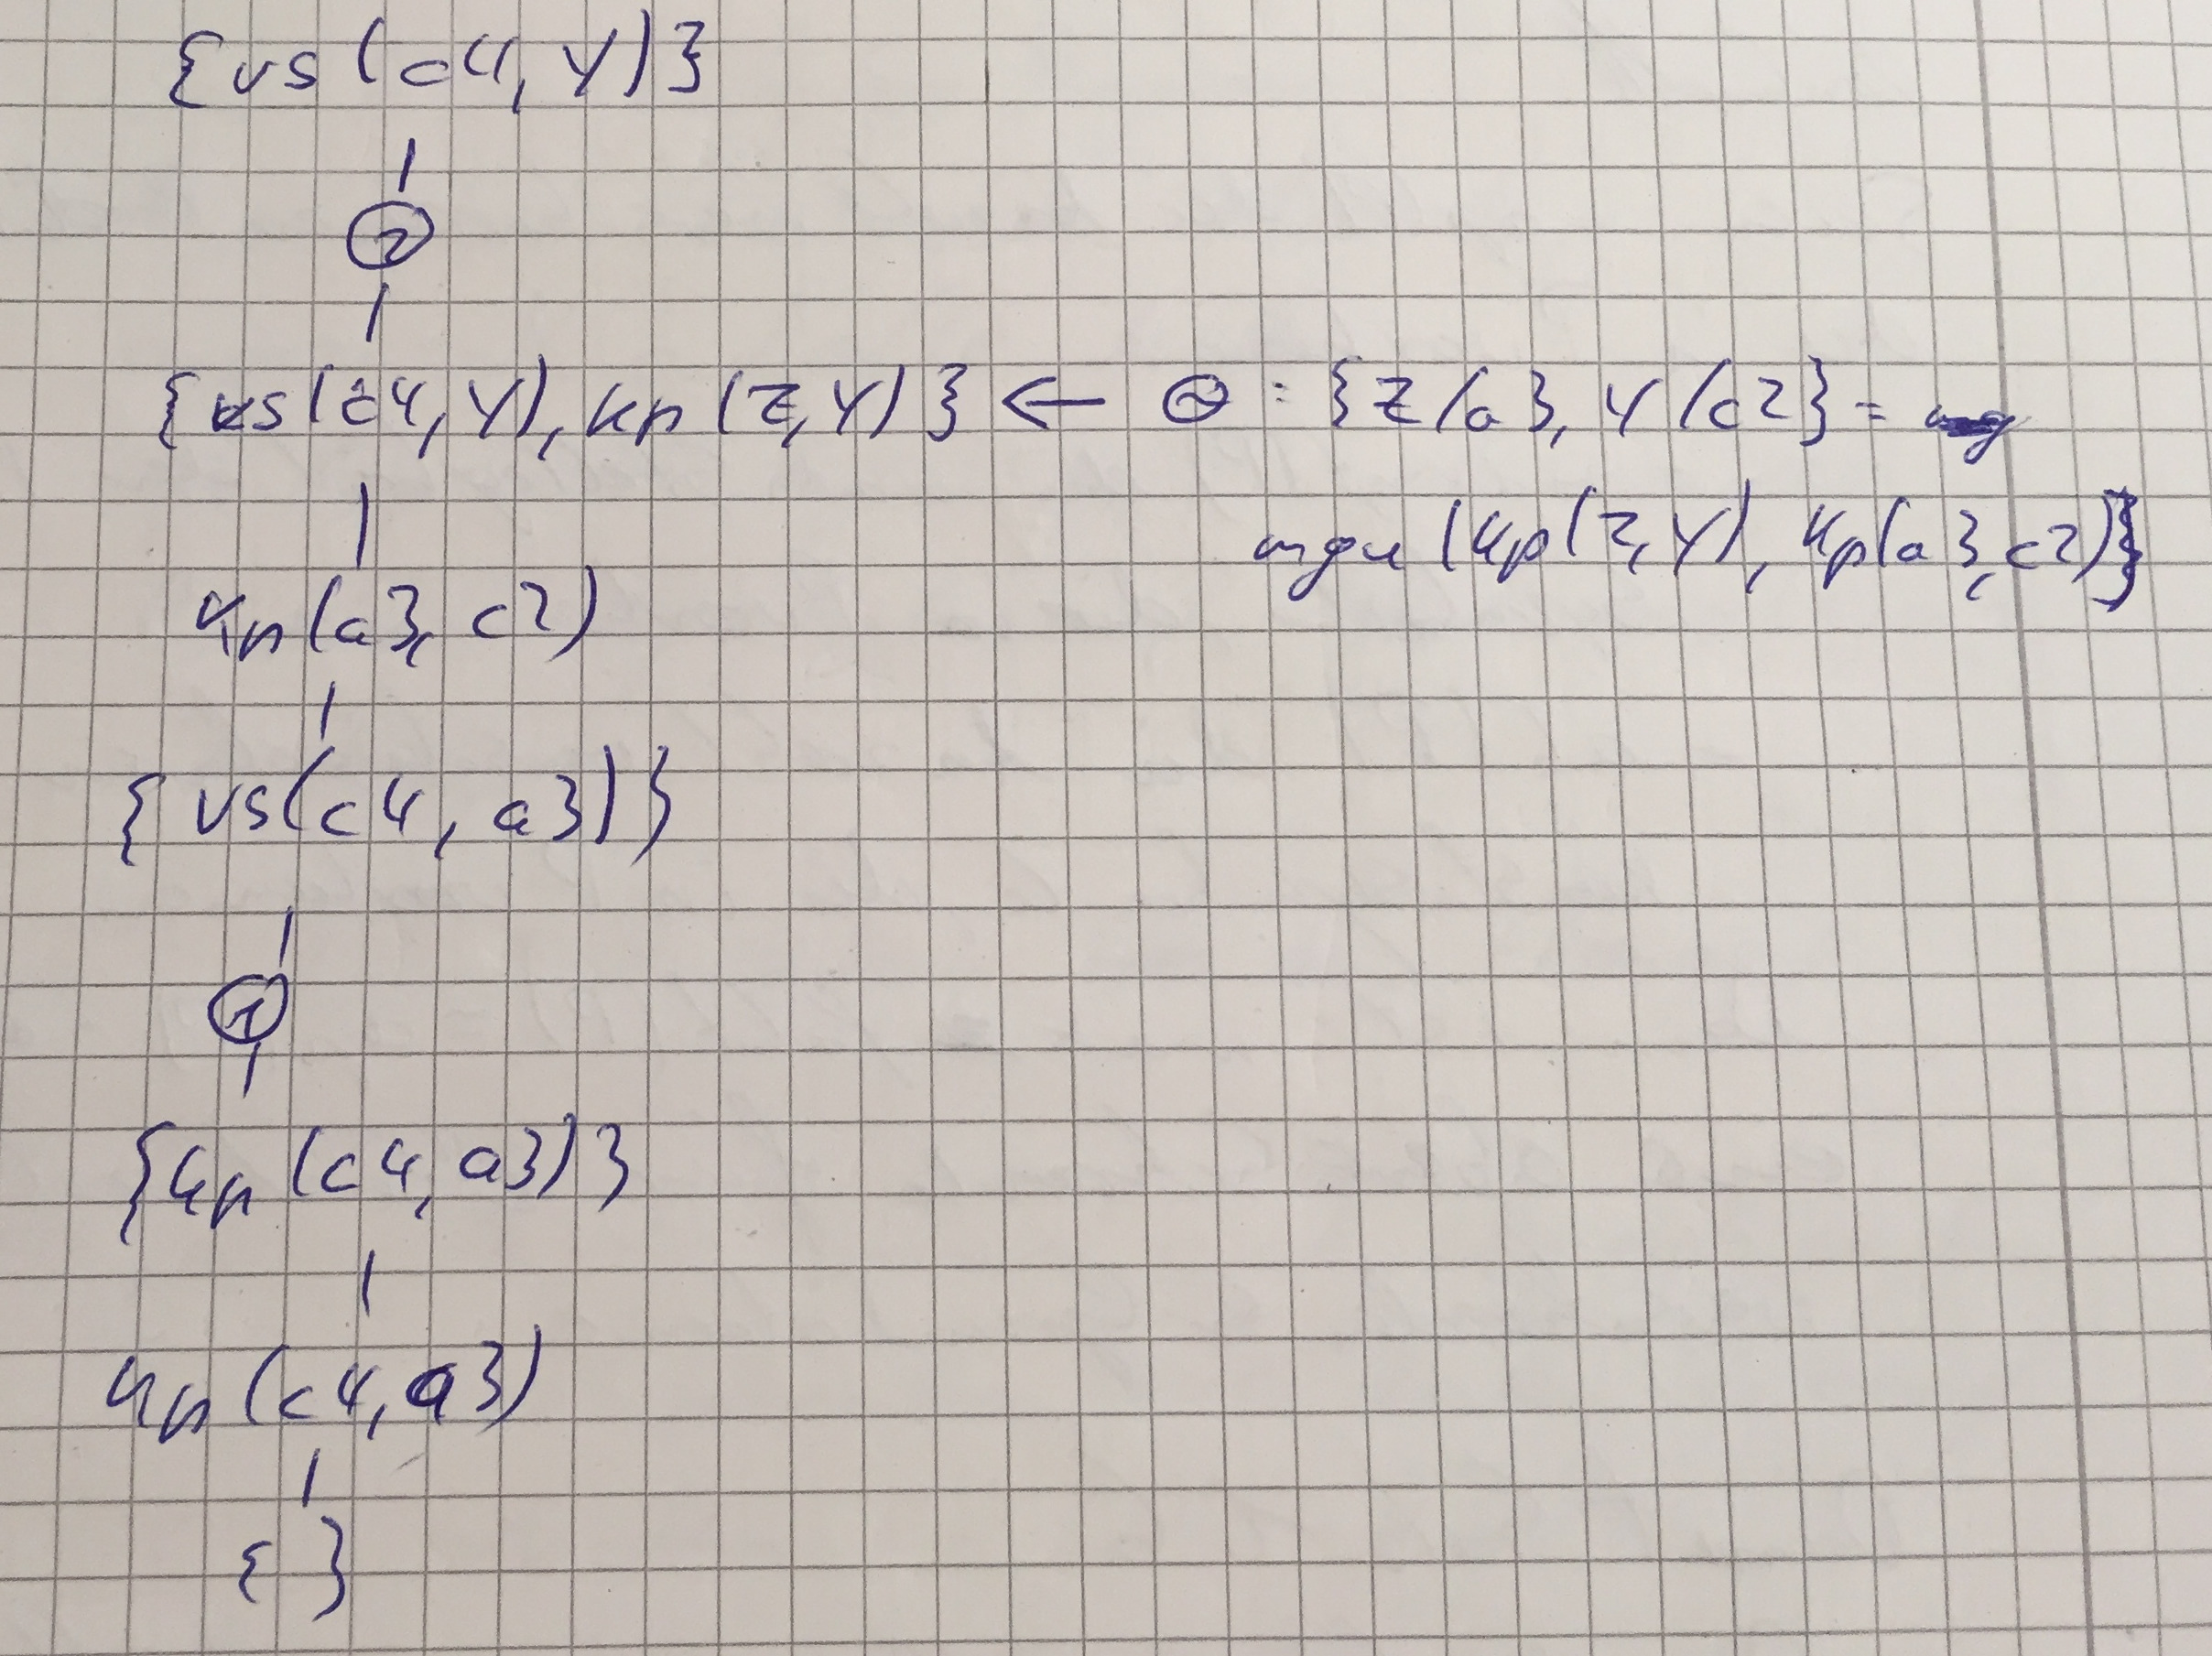
\includegraphics[width=0.7\linewidth]{img/img9}
\caption{}
\label{fig:img9}
\end{figure}


Seien $E = \{ \lnot M_1, \cdots, \lnot M_i, \cdots, \lnot M_K \}, r = L_0 :- L_1, \cdots, L_m$ eine Regel und $S(E) = \lnot M_i$. Es existiere $mgu(M_i, L_0) = 0$.
\paragraph{Resolvente von E und r:} $\{ \lnot M_1\Theta, \cdots, \lnot M_{i-1}\Theta, \lnot L_1 \Theta, \cdots, \L_m \Theta \lnot M_{i + 1} \Theta, \cdots, \lnot M_K\Theta \}$
\begin{itemize}
\item Unerfüllbarkeit: Anwendung der Methode ende mit $\square$ (leere Klausel, entspricht Falsch)
\item Ergebnis: Sei $g = \{ \lnot p(t_1, \cdots, t_n) \}$ das Ziel, $\{ p(t_1, \cdots, t_n)\Theta / \Theta$ Antwortsubstitution für eine Ableitung von g, die mit $\square$ endet \}



Ohne Beweis.

\subsection*{Satz 1.7}
Die SLD-Resolution liefert korrekte und vollständige Ergebnisse für alle Datalog-Programme.

\begin{figure}
\centering
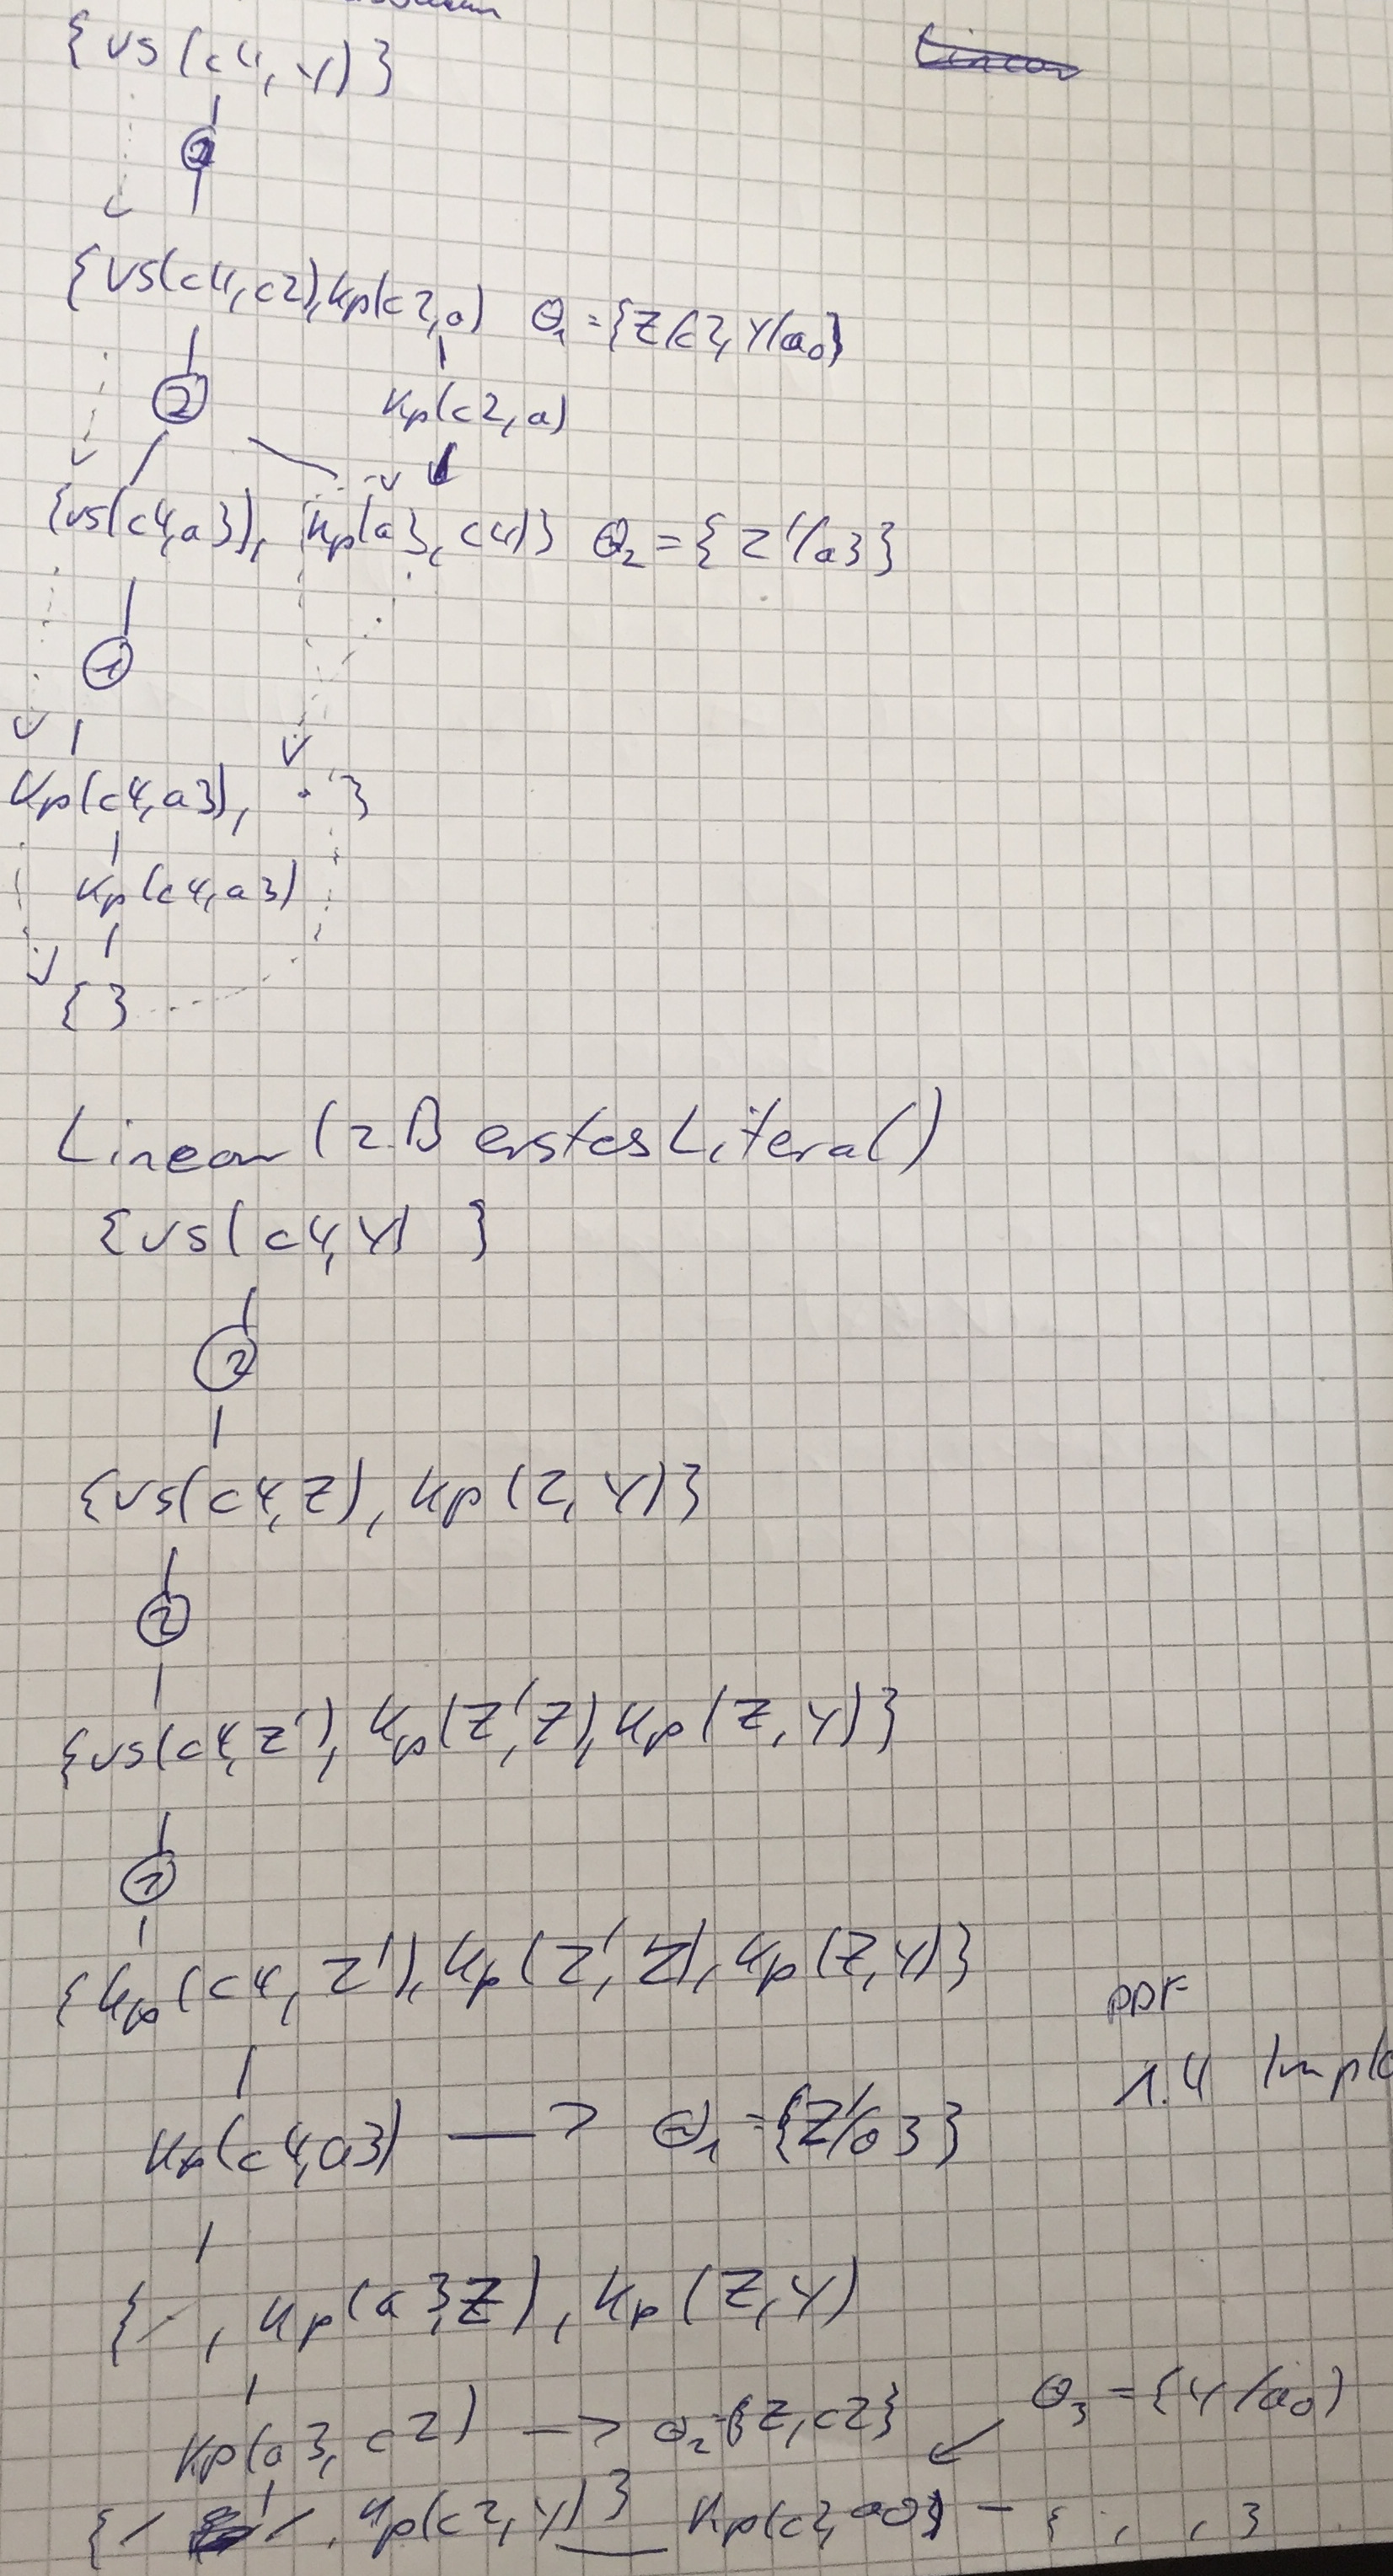
\includegraphics[width=0.7\linewidth]{img/img10}
\caption{}
\label{fig:img10}
\end{figure}
\begin{figure}
\centering
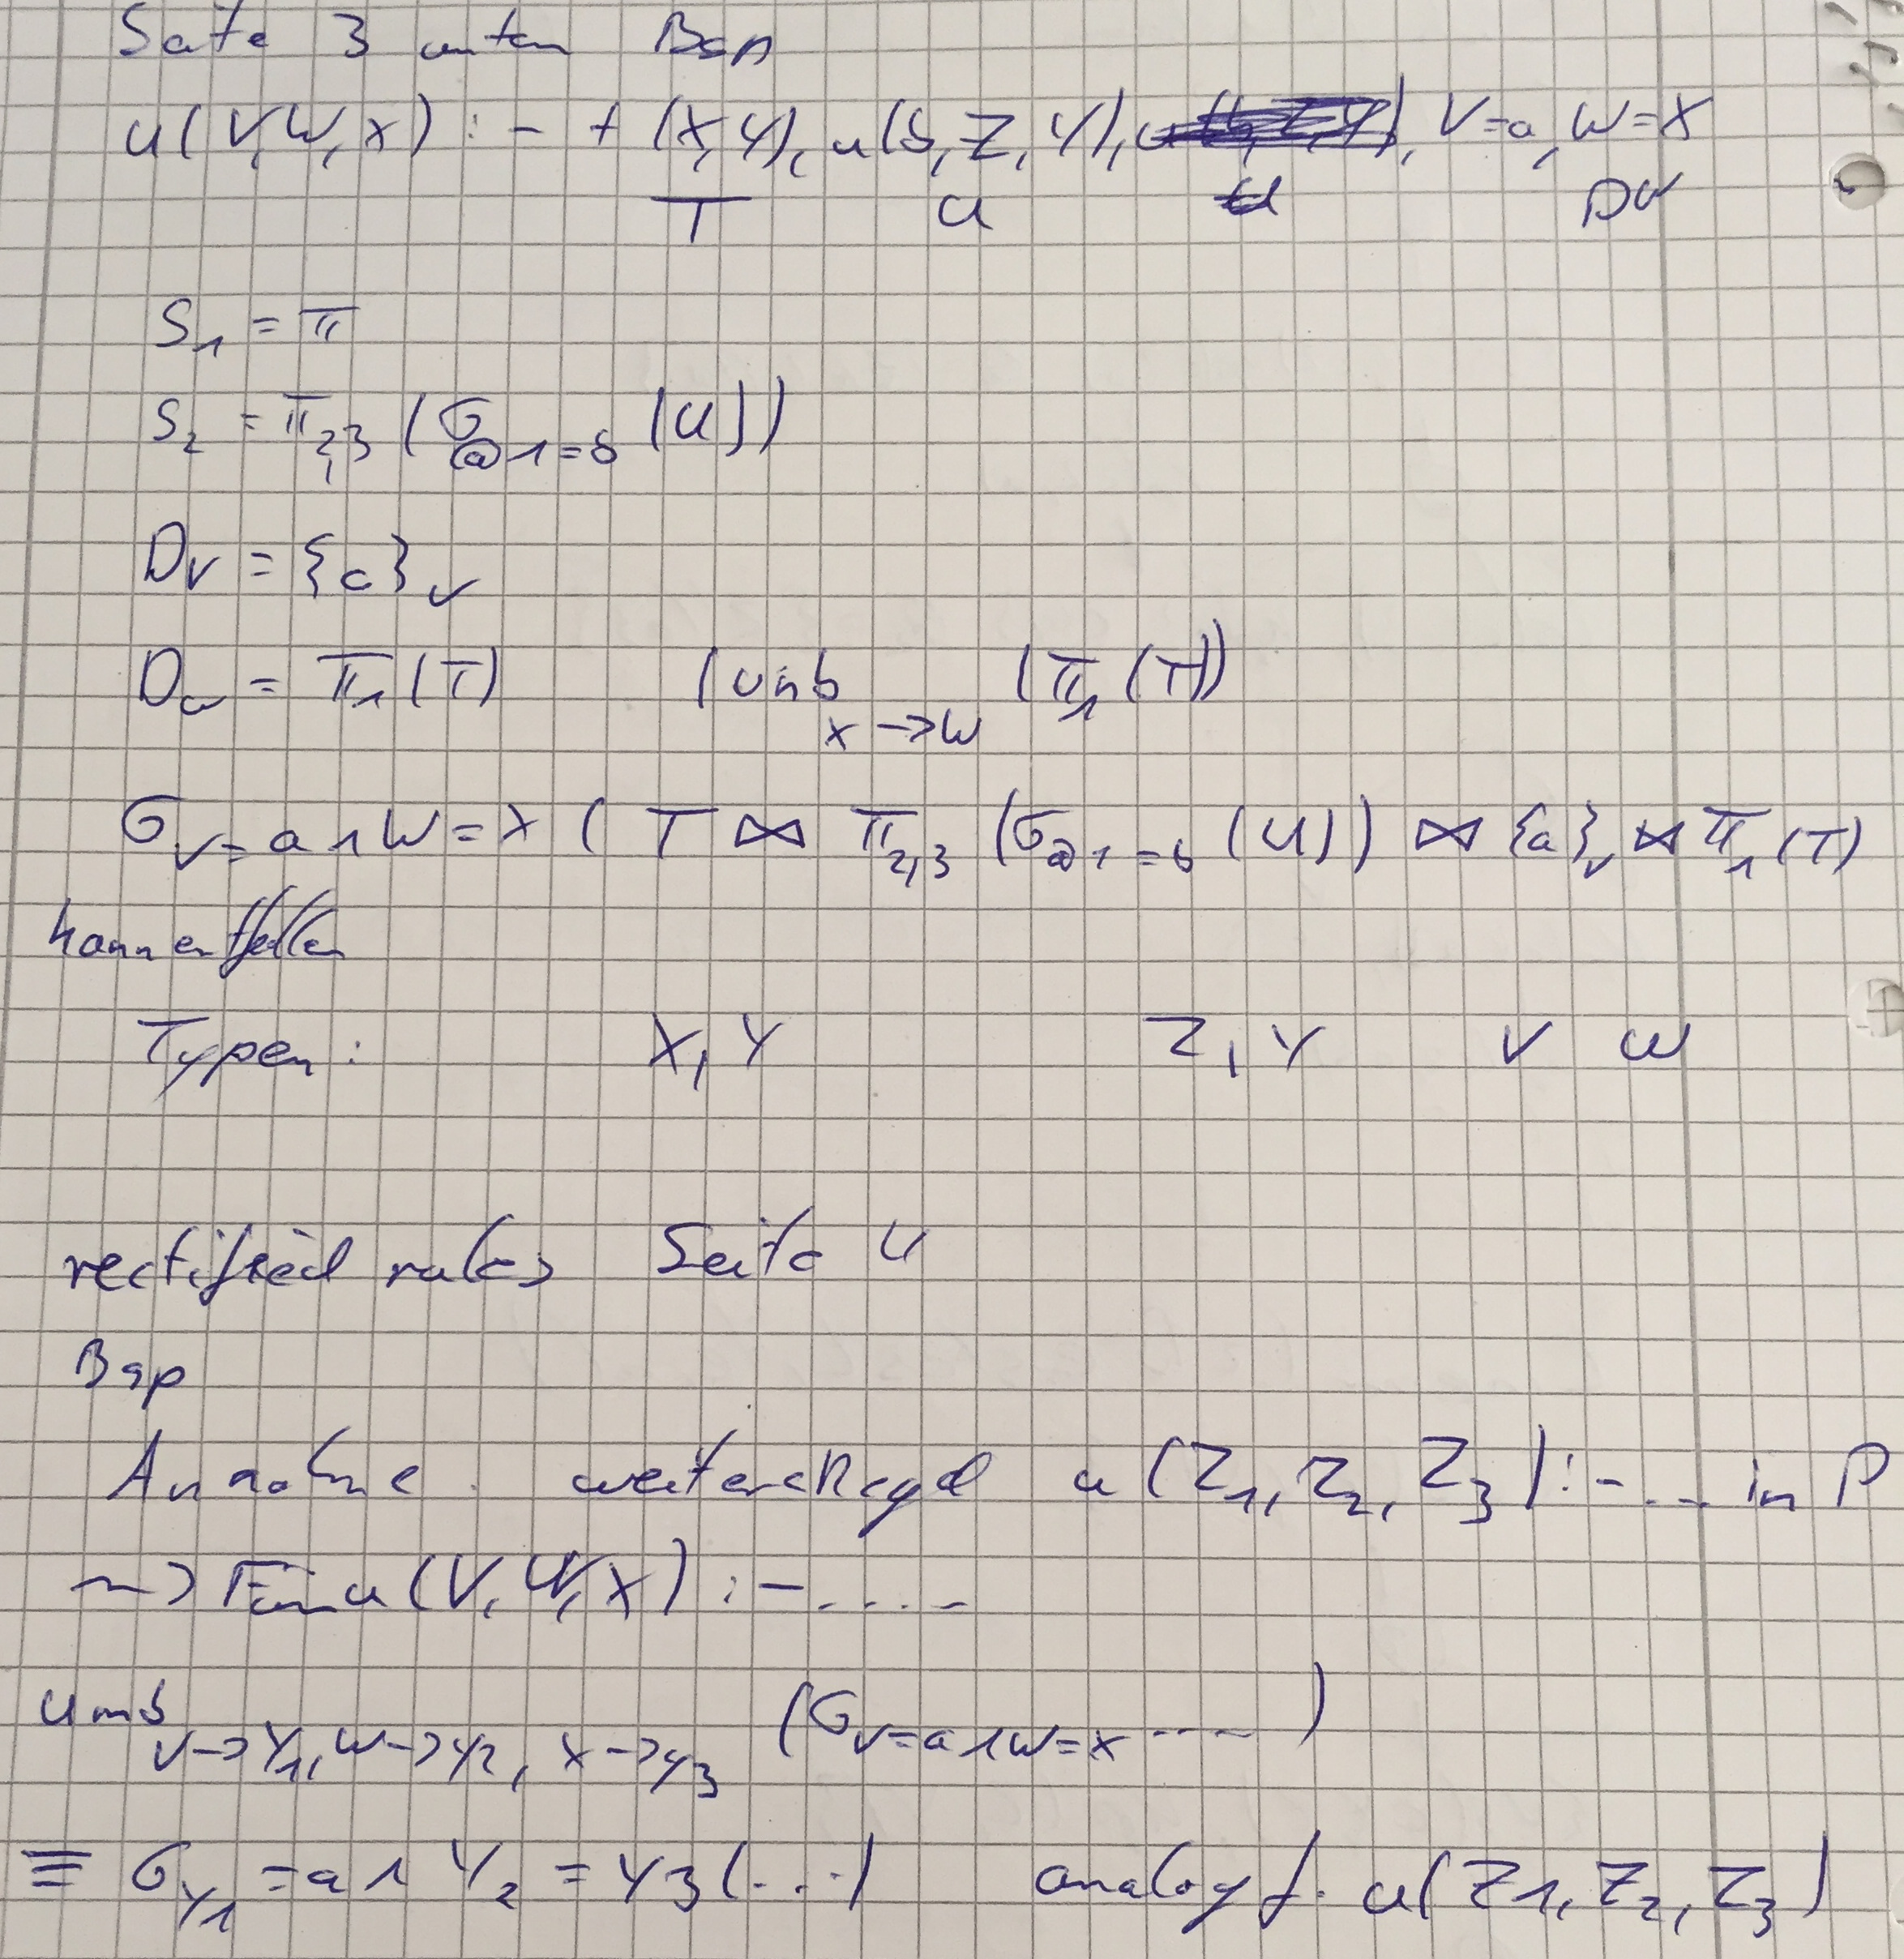
\includegraphics[width=0.7\linewidth]{img/img11}
\caption{}
\label{fig:img11}
\end{figure}
\end{itemize}


\paragraph{Beispiel} m alle Kurse $\neq$ a3 mit ihren Studierenden, die Voraussetzung von c4 sind.

\begin{align*}
r_1 = &vs(X,Y) :- Kp(X,Y). \\
&vs(c4, Y) :- vs(v4,Z), Kp(Z,Y). \\
&m(Z,W) :- vs(c4,Z), ag(Z,X), bl(Z,W,U), Z \neq a3.
\end{align*}

\paragraph{1.Schritt}
\begin{itemize}
\item $r_1$ \checkmark
\item $r_2 \leadsto \tilde{r_2} = vs(Q,Y) :- vs(C4,Z), kp(Z,Y), Q = c4.$
\item $r_3$ \checkmark
\end{itemize}

\paragraph{2.Schritt}
\begin{itemize}
\item $E_{r_1}$ = KURSPLAN
\item $E_{r_2} = \sigma_{Q = c4} \underbrace{\Pi_2 (\varsigma_{@1 = c4}(VS)}_Z \bowtie\footnote{Join Operation} \underbrace{KURSPLAN}_Z,Y \bowtie \underbrace{\{c4\}_Q)}_Q$
\item $E_{r_3} = \sigma_{Z \neq a3} \underbrace{\Pi_2 (\varsigma_{@1 = c4}(VS)}_Z \bowtie ANGEBOT \bowtie BELEGUNG$
\end{itemize}

\paragraph{3.Schritt}
vereinfacht $Q \Rightarrow X$\footnote{kommt nicht im Rumpf von $\tilde{r_2}$ vor}, damit $\tilde{r_1}$ und $\tilde{r_2}$ passen.
\begin{align*}
&vs(X,Y) \\
&vs(X,Y) \\
&m(Z,W)
\end{align*}


\paragraph{4.Schritt}
\begin{align*}
&VS = \underbrace{KURSPLAN}_{X Y} \cup \underbrace{(\Pi_2 (\varsigma_{@1 = c4}(VS)) \bowtie KURSPLAN \bowtie \{ c4 \}_X)}_X Y \\
&M = (\varsigma_{Z \neq a3}(\Pi_2 (\varsigma_{@1 = c4}(VS)) \bowtie ANGEBOT \bowtie BELEGUNG))[z,w]
\end{align*}

\subsubsection{Schreibweise für Gleichungssysteme}

\begin{align*}
&R_i = E_i \underbrace{(R_1, \cdots, R_n)}_{DB-Relationen}, i = 1, \cdots, n
\end{align*}


Vergleich der Ausruckskraft\footnote{genauere Definition später} von Datalog und Relationale Algebra:

\begin{itemize}
\item Reines Datalog ohne Rekursion entspricht $RA^+$ (monotone Relationale Algebra)
\item Reines Datalog ohne Rekursion entspricht $RA^+$ ohne Gleichungssysteme (> $RA^+$)
\end{itemize}

\paragraph{Beispiel:}

Kursplan (kp): \\
\begin{tabular}{|c|c|}
\hline
X & Y\\ \hline
c4 & a3 \\
a3 & c2 \\
c4 & a2 \\
c2 & a0 \\
\hline
\end{tabular}


\begin{align*}
&vs(X,Y) :- Kp(X,Y).
&vs(X,Y) :- \underbrace{vs(X,Z)}_{X Z}, \underbrace{kp(Z,Y)}_{Z Y}.
&\leadsto vs = \Pi_{1,3}(VS \bowtie KURSPLAN) \cup KURSPLAN
\end{align*}

Jacobs entspricht Gauss-Seidel

\begin{align*}
R^0 &= \emptyset \\
Q^1 &= \emptyset \\
R^1 &= KP \quad \leftarrow (\emptyset_{X2} \bowtie KP_{ZY}) [X,Y] \\
Q^2 &= KP \\
R^2 &= \{ (c4,c2), (a3,a0) \} \cup KP \quad (KP_{XZ}) \bowtie KP_{ZY})[X,Y] \cup KP_{X,Y} \\
Q^3 &= R^2 \\
R^3 &= \{(c4,a0)\} \cup R^2 \quad (((KP_{XZ} \bowtie KP_{ZY}\footnote{Es wird zu viel berechnet beim Join. Siehe unten})[X,Y] \cup KP_{XY})_{XZ})[X,Y] \cup KP_{XY}  \\
\end{align*}

\subsubsection{Anmerkung}
Berücksichtigung der ``neuen'' Information für VS hätte genügt. Grund: $(VS' \cup VS'') \bowtie KURSPLAN = VS' \bowtie KURSPLAN \cup VS'' \bowtie KURSPLAN $

\paragraph{Nach Schritt 4}

\begin{align*}
&R_1 \bowtie R_2 \cup R_2 \bowtie R_3 \Rightarrow^{mit \delta - Beruecksichtigung} \footnote{Ist suboptimal, weil wieder zu viel brerchnet wird} \\
& \delta R_1 \bowtie \cup R_2 \bowtie R_3 \cup R_1 \bowtie \delta R_2 \cup \delta R_2 \bowtie R_3 \cup R_1 \bowtie R_2 \cup R_2 \bowtie \delta R_3 \\
&\Rightarrow\footnote{Ist besser} \delta R_1 \bowtie R_2 \cup R_1 \bowtie \delta R_2 \cup \delta R_2 \bowtie R_3 \cup R_w \bowtie \delta R_3
\end{align*}

\begin{align*}
& \delta R^0 = KP \\
& R^0 = KP \\
& \delta Q^1 = KP \\
& \delta R^1 = \{ (c4,c2), (a3,a0)\} \cup KP \\
& \delta R^1 = \{ (c4,c2), (a3,a0)\} \cup KP \\
& R^1 = Kp \cup \{(c4,c2), (a3,a0)\} \\
& \delta Q^2 = \{(c4,c2), (a3,a0)\} \\
& \delta R^2 =  \delta Q^2 \bowtie Kp \cup Kp = \{(c4,a0)\}  \cup Kp \\
& R^2 =  Kp \cup \{ (c4,c2), (a3,a0) \} \cup \{(c4,a0)\} \\
& \delta Q^3 = \{(c4,a0)\} \\
& \delta R^3 = \delta Q^3 \bowtie Kp \cup Kp = Kp \\
& \delta R^3 = \emptyset \\
& R^3 =  R^2 \cup \emptyset
\end{align*}

\begin{figure}
\centering
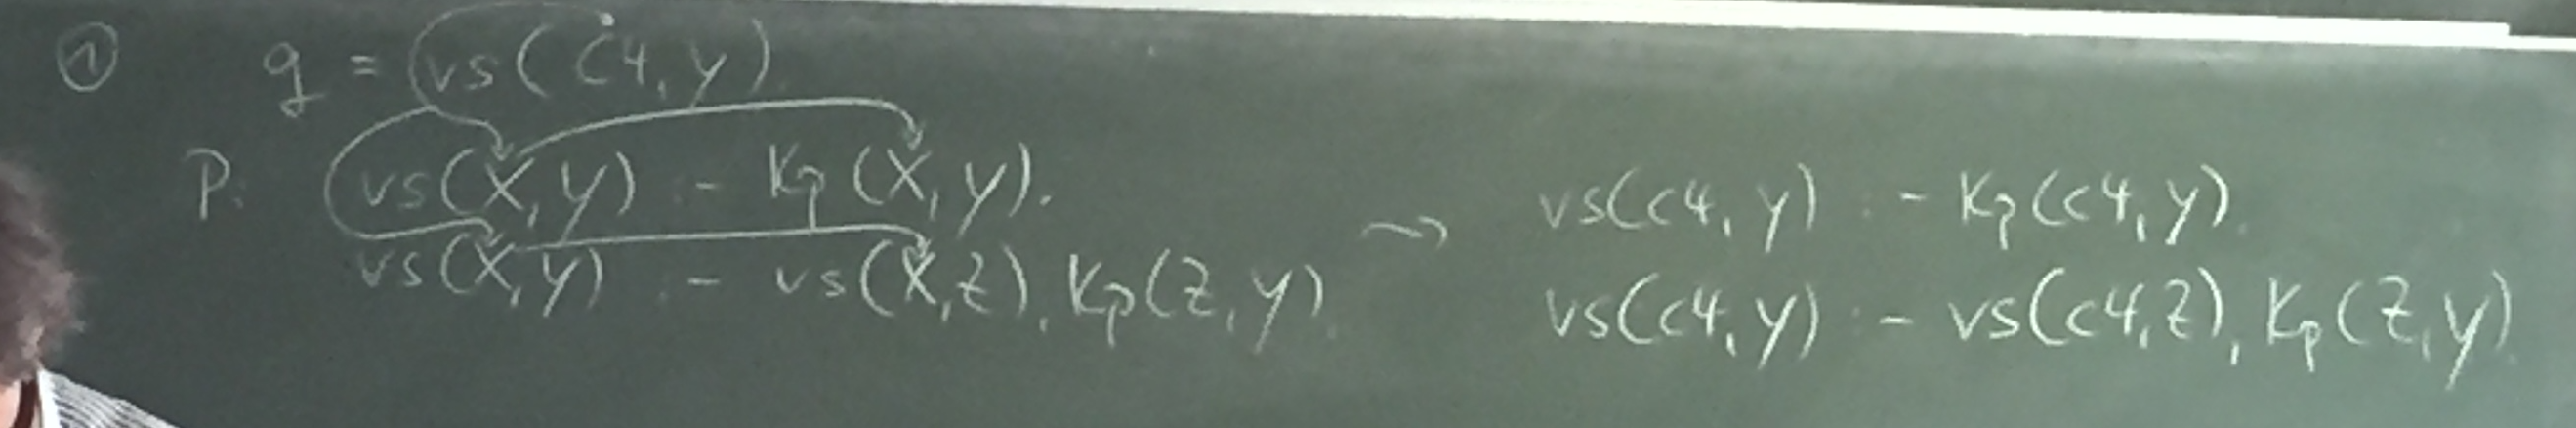
\includegraphics[width=0.95\linewidth]{img/img12}
\caption{}
\label{fig:img12}
\end{figure}

\begin{figure}
\centering
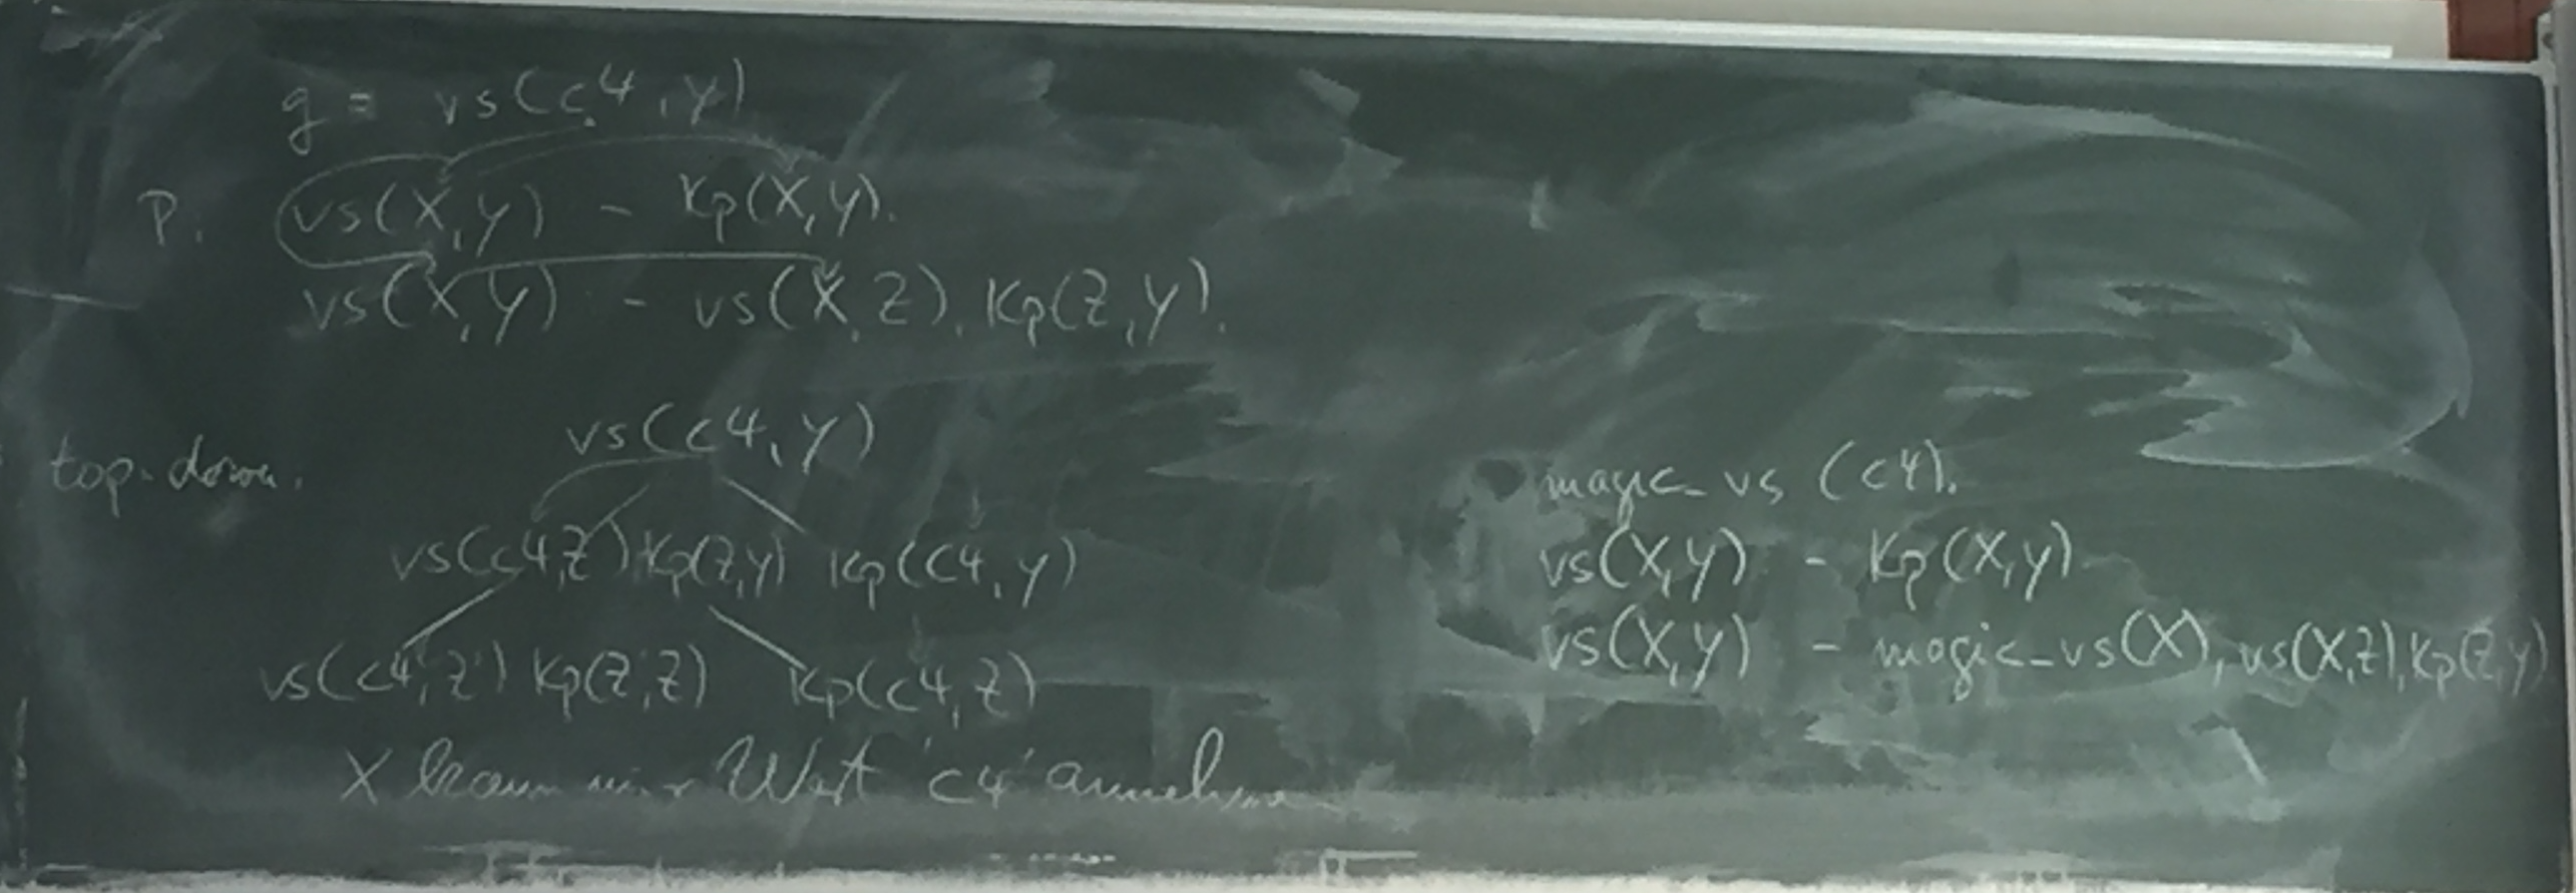
\includegraphics[width=0.95\linewidth]{img/img13}
\caption{}
\label{fig:img13}
\end{figure}

\begin{figure}
\centering
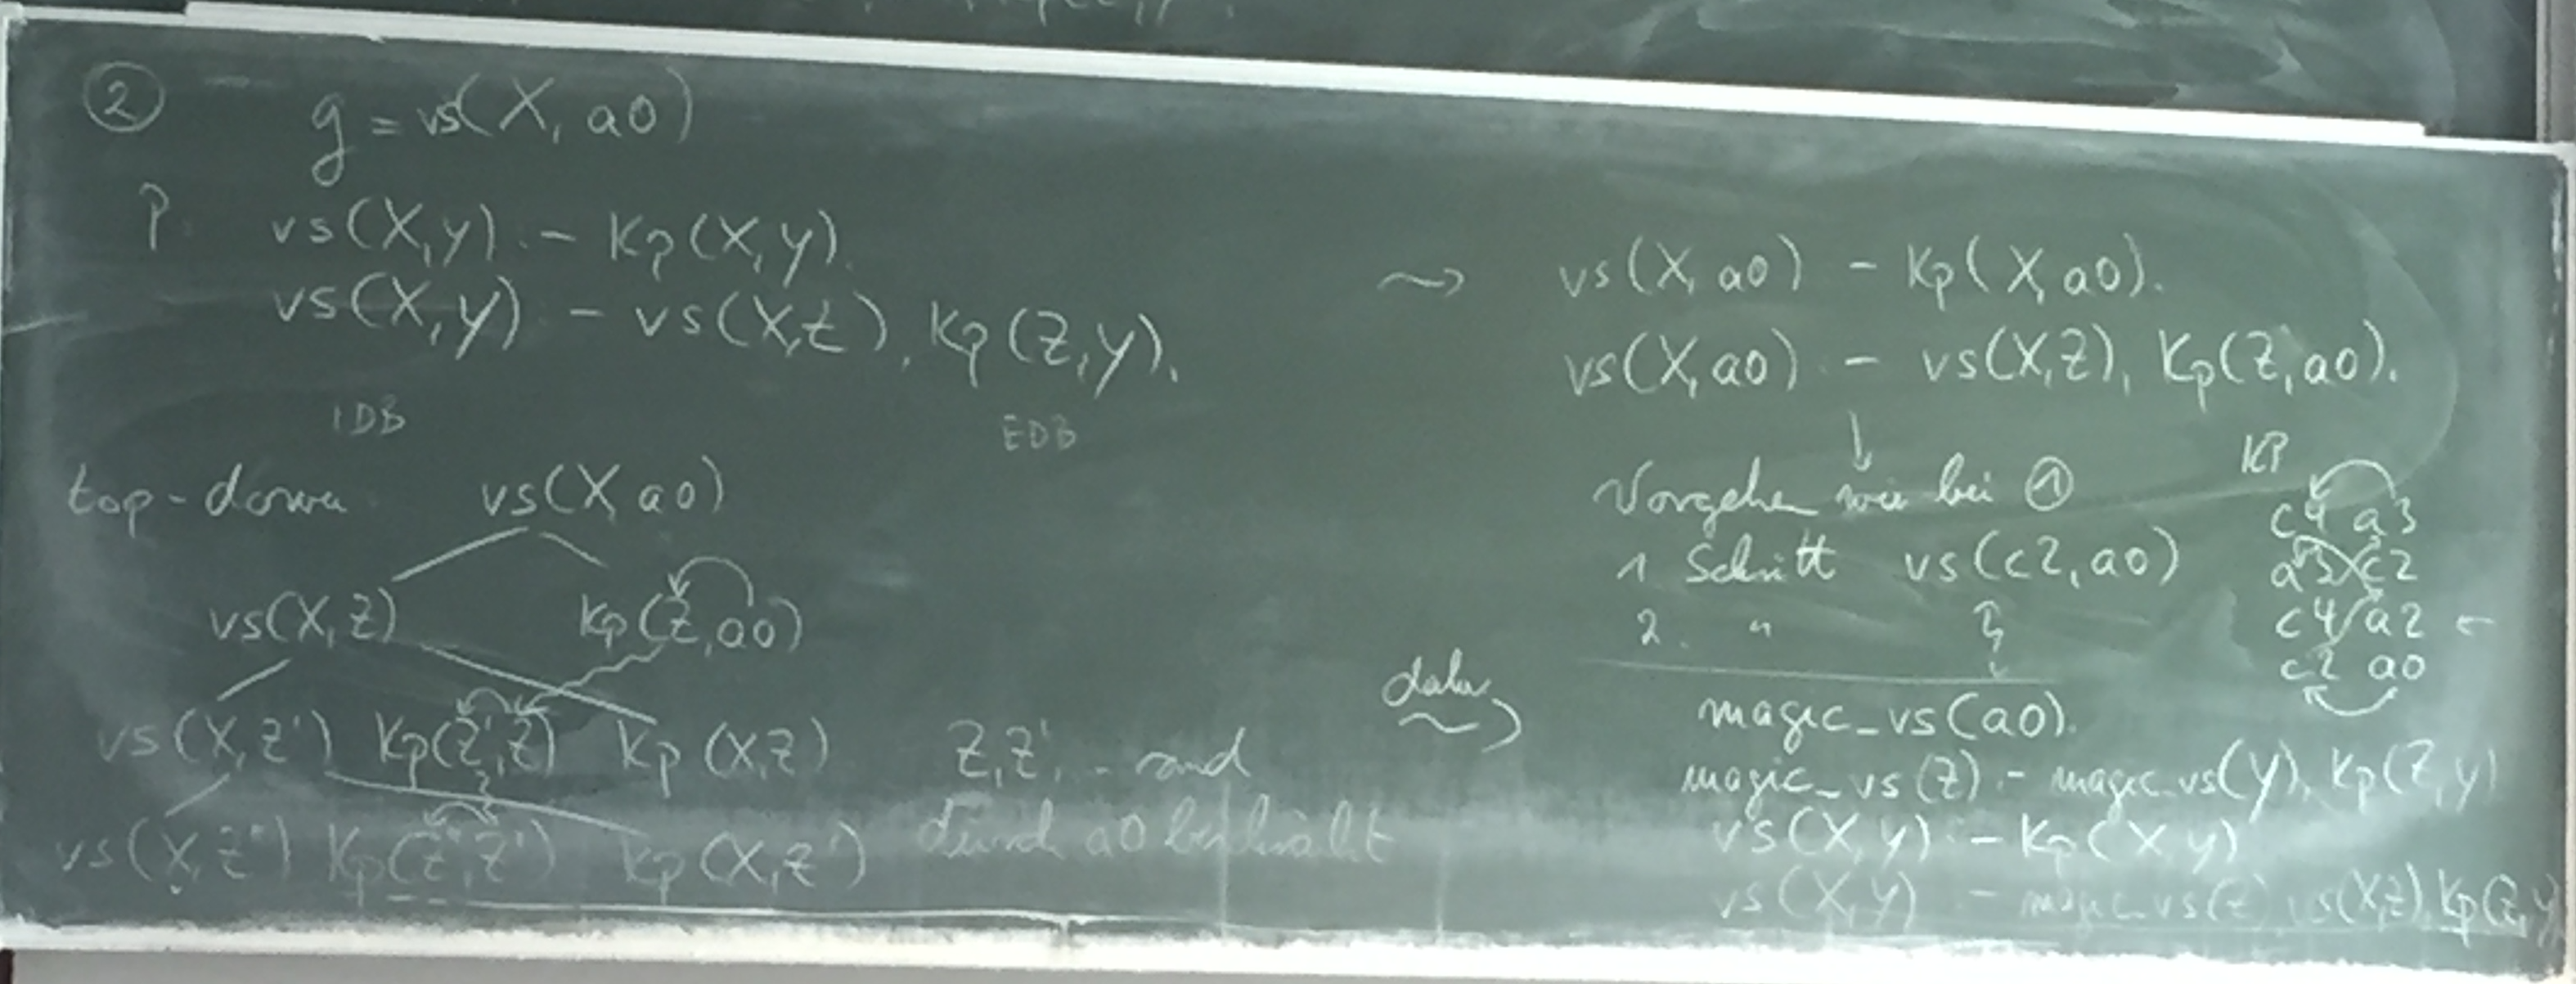
\includegraphics[width=0.95\linewidth]{img/img14}
\caption{}
\label{fig:img14}
\end{figure}

\paragraph{Beispiel}

\begin{align*}
&r_2 = vs^{fb}(X,Y) :- vs^{fb}\_(X,Z), Kp(Z,Y). \\
&i) \checkmark \\
&ii) \cdots magic\_r_2\_vs^{fb}\_1(X,Z) \cdots \\
&iii) \cdots magic\_r_2\_vs^{fb}\_1(Z) \cdots \\
&iv) vs^{fb}(Y)\\
& magic\_r_2\_vs^{fb}\_1(Z) :- magic\_vs^{fb}(Y), kp(Z,Y).
\end{align*}


\begin{align*}
&r_0 = query^f(X :- vs^{fb}\_(X,a0). \\
&i) \cdots \\
&ii) query^f(X) :- magic\_r_0\_vs^{fb}\_1(X,a0) \\
&iii) query^f(X) :- magic\_r_0\_vs^{fb}\_1(a0) \\
&iv) - \\
&v) vs^{fb}(Y)\\
& magic\_r_0\_vs^{fb}\_1(a0) :- magic\_query^f().\\
r_0 &\leadsto\footnote{``Sideways information passing''} magic\_r_0\_vs^{fb}\_1(a0) :- . \\
r_2 &\leadsto magic\_r_2\_vs^{fb}\_1(Z) :- magic\_vs^{fb}(Y), Kp(Z,Y).
\end{align*}

\begin{align*}
&p(X):- \lnot q(X) \\
&p(X) \cup q(X) \\
&q(X) :- \lnot p(X)
\end{align*}

$P = \{ ag(a3, o) :- \lnot ag(a3,m) \}.$ \\
``Falls `m' Kurs a3 nicht anbietet, bietet o den Kurs an'' \\
Mit CWA: 

\begin{align*}
&ag(a3,m) \not\in ANGEBOT \\
&ag(a3,o) \not\in ANGEBOT
\end{align*}

Da beide keine logische Folgerung von P (müsste in allen Modellen gültig sein) Nimm Modelle $\{ ag(a3, o) \}$.

\begin{align*}
&\{ ag(a3, o) \} \\
& \Rightarrow^{CWA\footnote{Closed World Assumption}} \lnot ag(a3, m) \text{ und } \lnot ag(a3, o) \text{ sind gültig.} \\
& \text{Aber } \lnot ag(a3,m) \Rightarrow ag(a3,0) \leadsto \text{Wiederspruch zur CWA}
\end{align*}


Beachte folgende HB-Interpretation von P.

\begin{align*}
&I_1 = \{ ag(a3, o) \} \text{ und } I_2 = \{ ag(a3, m) \} (I_1, I_2 \text{ sind minimale Modelle}) \\
&I_3 = \{ ag(a3, o), ag(a3,m) \} \text{ ist ebenfalls Modell von P}
\end{align*}

In $I_1$ gilt mit CWA: $\lnot ag(a3,m)$ \\
In $I_2$ gilt mit CWA: $\lnot ag(a3,o)$ \\

\paragraph{Grund für Problem:} Implikation $\lnot ag(a3,m) \Rightarrow ag(a3, o)$ äquivalent zu $ag(a3,m) \vee ag(a3, 0)$. Welches Modell soll ausgezeichnet werden? Semantik?

\paragraph{Offensichtlich:} I Modell von P $\diamondsuit$ I Modell von $P' = \{ ag(a3,m) :- ag(a3, o)\}$
Gehe wie bei Fuxpunktberechnung vor:

\paragraph{P}
Bekannte Fakten $EDB = \{ ag(a1,m)\, ag(c4,q), ag(a3,d), \cdots \}$ \\
$ag(a3, m) \not \in EDB$ \\
CWA: $\lnot ag(a3, m) \text{ gilt} \Rightarrow^{\text{Regel}} ag(a3,0)$ \\

\paragraph{P'}
$ag(a3, o) \not \in EDB$ \\
CWA: $\lnot ag(a3, 0) \text{ gilt} \Rightarrow^{\text{Regel}} ag(a3,m)$ \\

Daraus folgt: Wähle $I_1(I_2)$ als Modell (Semantik) von P(P') $\leadsto$ Auswertungsrichtung gemäß Implikation legt Semantik fest. D.h. Semantik ist abhängig von der Art des Aufschreibens der Klauseln. Daraus ergibt sich die Frage nach einer besseren Semantikdefinition.

% TODO: BILD HIER

\begin{align*}
r(1), s(1), s(2).& \\
U(X) :- r(X). r(1) \leadsto u(1)& \\
q(X) :- s(X), \lnot u(X).& \Leftarrow s(1) \leadsto q(1)\\
& \Leftarrow s(2) \leadsto q(2)
\end{align*}

\end{document}